% \newcommand{\prototitle}{Versuch 2 - Statistik}
% \newcommand{\Fachbereich}{Praktikum Messtechnik}
% \input{../packages/tu_header}

\newcommand{\institut}{Institut f\"ur Telekommunikationssysteme}
\newcommand{\fachgebiet}{Nachrichten\"ubertragung}
\newcommand{\veranstaltung}{Praktikum Nachrichten\"ubertragung}
\newcommand{\pdfautor}{\"Ozg\"u Dogan (326 048), Boris Henckell (325 779)}
\newcommand{\autor}{\"Ozg\"u Dogan (326 048)\\ Boris Henckell (325 779)}
\newcommand{\gruppe}{Gruppe: D03}
%\newcommand{\betreuer}{Betreuer: Mahmoud Felk}


\newcommand{\pdftitle}{Nachrichten\"ubertragung\ Praktikum\ 04}
\newcommand{\prototitle}{Praktikum 04 \\ Pulsamplitudemodulation und nichtideale Abtastung}


\input{../../packages/tu_header_8}
%\begin{document}

% \lstlistoflistings
\definecolor{darkgray}{rgb}{0.95,0.95,0.95}
\definecolor{darkolivegreen}{HTML}{01a801}
\definecolor{functionsBlue}{HTML}{32b9b9}
\definecolor{variableRed}{rgb}{1,0,0}
\definecolor{stringBrown}{HTML}{bc8e8e} % f geht nicht

\lstset{
        %\lstset{extendedchars=true} % Umlaute an der richtigen stelle und nicht am Anfang ausgeben
        %basicstyle=\footnotesize\ttfamily,
        basicstyle=\small,
        %
        inputencoding=utf8,
        %
        tabsize=4,
        showspaces=false,
        showtabs=false,
        showstringspaces=true, % no special string spaces
        %
        backgroundcolor=\color{darkgray}, % background
        stringstyle=\color{stringBrown}\fseries, % Strings
        keywordstyle=\color{functionsBlue}\bfseries, % keywords Blau
        identifierstyle=\color{variableRed}, % variablen
        commentstyle=\color{darkolivegreen}, %  comments
        %
        breaklines=true,
        %
        numbers=left,
        numberstyle=\tiny,
        stepnumber=1,
        numbersep=7pt,
        %
        frame=single,
        columns=flexible,
        %
        xleftmargin=-2cm,
        xrightmargin=-1.5cm,
        %
        language=Matlab
}

%---------------------------------------------------------------------
%---------------------------------------------------------------------
%---------------------------------------------------------------------


\section{Einleitung}
\begin{quote}
	\TODO{Einleitung so okay?}\\
	In diesem Termin werden zwei nichtideale Abtastverfahren für die
	Rekonstruktion eines PAM-modulierten Signals untersucht. Diese zwei Verfahren
	sind die Abtastung durch Signalausblendung (shape-top sampling) und die
	Abtastung mit Signalverbreiterung (flat-top sampling). Beide Verfahren werden
	im Zeit- und im Frequenzbereich untersucht, dabei werden ihre Auswirkungen auf
	die Rekonstruktion der abgetasteten Signale interpretiert.
\end{quote}%beende Einleitung
%--------------------------------------------------------------------
%--------------------------------------------------------------------    

\section{Motivation}
\begin{quote}
	Die in diesem Praktikum behandelte Pulsamplitudenmodulation hat das Ziel aus
	einem zeitkontinuerliches Signal kleine Zeitabschnitte auszuschneiden, die dann über einen Nachrichtenkanal übertragen
	werden kann um später wieder demoduliert das Ursprungssignal zu ergeben. Der
	Sinn und Zweck dieser Modulation ist, wie auch bei der Frequenzmodulation und der Amplitudenmodulation, 
	mehrere Signale gleichzeitig über einen Kanal zu übertragen. Die Pulsamplitudenmodulation ist in
	diesem Fall die nötige Vorstufe für das Time-Division-Multiplexen, bei dem mehrere Signale zu verschiedenen Timeslots
	über einen Kanal versendet werden.\\
	Die beiden verwendeten Verfahren der Pulsamplitudenmodulation haben jeweils Vor und Nachteile, die im folgenden näher
	erläutert werden.
\end{quote} %section

%--------------------------------------------------------------------
%--------------------------------------------------------------------    


\section{Theorie}
\begin{quote}
	\subsection{Abtastung durch Signalausblendung (shape-top sampling)}
    \begin{quote} 
        Bei dem Shape-Top sampling wird das Originalsignal mit einer Rechteckfolge multipliziert. Die Rechtecke dieser
        Folge haben die Breite $\alpha \cdot T$ mit einem $\alpha \leq 1$ und sind somit schmaler als die Abtastzeit
        $T$. Daraus resultiert, ein nichtideal abgetastetes Signal. Die Dächer der ausschneidenden Rechtecke
        beinhaltet den originalen Verlauf des Nutzsignals. Im folgenden Bild ist das Prinzip des
        Shape-Top sampling veranschalicht.\\

        \begin{figure}[H]
        \centering
            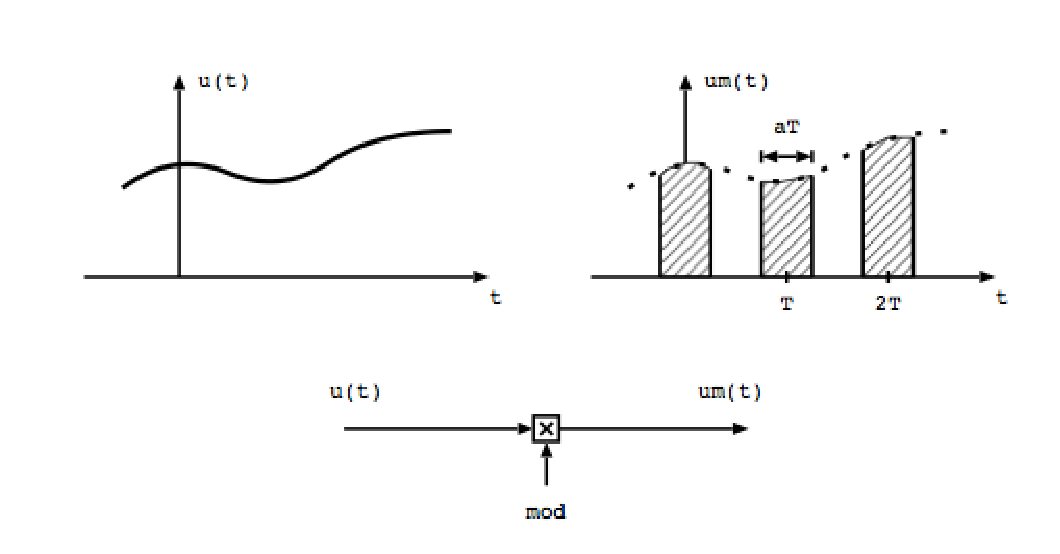
\includegraphics[scale=0.6, trim = 0cm 0cm 0cm 0cm, clip]{./Bilder/PrinzipSignalausblendung}
                \caption{Prinzip der Signalausblendung}
                \cite{PrinzipSignalausblendung}
        \end{figure}
    
        Pratisch lässt sich diese Art der Modulation durch einen Schalter realisieren, der jeweils nur
        kurzzeitig geschlossen wird.\vspace{1em}
        
        Das oben erwähnte $\alpha$ bezeichnet in diesem Fall das
        Tastverhältniss. Es beschreibt den Prozentsatz wie breit ein Rechteck in Verhälltniss zur angegebenen halben 
        Periodendauer ist. Mit Hilfe dieses Wertes $\alpha$ lassen sich die Zeitfenster einstellen, 
        die ein Signal zur Verfügung haben soll. Sollen beispielsweise zwei Signale auf einem Kanal mit Hilfe 
        von Time-Devision Multiplexing übertragen werden wird das $\alpha =
        \frac{1}{2}$ gewählt und jedes der Signale hat die Hälfte der Zeit auf dem Kanal. Sollen wiederum auf dem selben 
        Kanal $100$ verschiedene Signale übertragen werden wird $\alpha = \frac{1}{100}$ und jedes Signal hat
        $\frac{1}{100}$ der Zeit auf dem Kanal.\vspace{1em}
        
        Interessant ist, welche auswirkung diese Art der modulation auf das Frequenzspekrum des Originalsignals hat.
        Dazu betrachten wir das Zeitsignal und transformieren es in den Frequenzbereich.
        
            \begin{equation*}
                \begin{split}
                    f_m (t)   &= f(t) \cdot \sqcap_{\alpha T} (t) \ast \delta_T (t) \\
                    F_S (j\omega) &= \frac{1}{2\pi} F (j\omega) \ast \left [
                    \alpha T \cdot si \left( \frac{\omega \cdot \alpha T}{2} \right) \cdot \omega_T \cdot \delta_{\omega
                    T} (\omega) \right] \\
                    &= \frac{1}{2\pi} F (j\omega) \ast \left [
                    \alpha \frac{2 \pi}{\omega_T} \cdot si \left( \frac{\omega \cdot \alpha T}{2} \right) \cdot \omega_T
                    \cdot \delta_{\omega T} (\omega) \right] \\
                    &= \alpha \cdot F (j \omega) \ast \left ( si \left( \frac{\omega \cdot \alpha T}{2} \right)
                    \sum_{k=-\infty}^{\infty} \delta (\omega - k\omega_T) \right)\\
                    &= \alpha \cdot F (j \omega) \ast \left ( si \left( \frac{\omega \cdot \alpha \frac{2
                    \pi}{\omega_T}}{2} \right) \sum_{k=-\infty}^{\infty} \delta (\omega - k\omega_T) \right)\\
                    &= \alpha \cdot F (j \omega) \ast \left ( si \left( \frac{\omega \cdot \alpha \pi}{\omega_T}
                    \right) \sum_{k=-\infty}^{\infty} \delta (\omega - k\omega_T) \right)\\
                    &= \alpha \cdot F (j \omega) \ast \sum_{k=-\infty}^{\infty} (si(k \pi \alpha) \cdot \delta (\omega -
                    k\omega_T))\\
                    &= \alpha \cdot \sum_{k=-\infty}^{\infty} \left [ si(k \pi \alpha) \cdot F (j(\omega - k\omega_T))
                    \right]\\
                \end{split}
            \end{equation*}
            
        Als Sonderfall sollte außerdem noch das Basisband ($k = 0$) erwähnt werden:
        
       \begin{equation*}
        	\begin{split}
        		U_m (j\omega) = \alpha \cdot U(j\omega)
        	\end{split}
        \end{equation*}        
        
        Diese Fourier-Transformation verdeutlicht, dass das gesamte Amplitudensprktrum im Frequenzbereich um den Faktor
        $\alpha$ dedämpft wird. Außerdem werden alle Bänder mit $k > 0$ zusätzlich um den Faktor $si(k \pi \alpha)$
        gedämpft. Falls das Produkt $k \cdot \alpha$ eine ganze Zahl und somit das Produkt innerhalb der $si()$ Funktion
        ein ganzzahliges vielfaches von $\pi$ ergibt wird dieses Frequenzband vollständig gedämpft. Die Amplituden eines
        einzelnen Frequenzbandes werden jedoch nicht unterschiedlich zueinander gedämpft.\\
        
        Die eben besprochenen Auswirkungen der Modulation auf das Amplitudenspekrum verdeutlicht auch das folgende Bild.
        
        \begin{figure}[H]
        \centering
            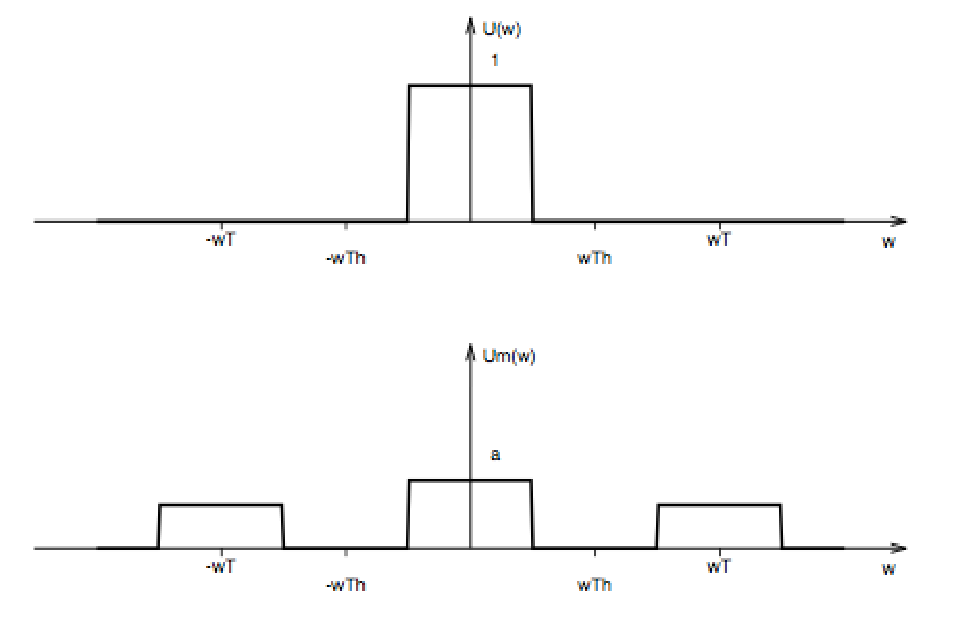
\includegraphics[scale=0.7, trim = 0cm 0cm 0cm 0cm, clip]{./Bilder/AmplitudenspektrumShap_Top}
                \caption{Amplitudenspektrum Shap_Top Sampling}
                \cite{AmplitudenspektrumShap_Top}
        \end{figure}
        
        Dieses Verhalten im Frequenzbereich ist ein großer Vorteil dieses Verfahrens der Pulsamplitudenmodulation. Die
        Amplitudenspektren werden zwar gedämpft jedoch beiben sie unverzerrt. Diese Dämpfung lässt sich beim Empfänger
        jedoch wieder durch eine Verstärkung kompensieren. Problematisch wird es erst wenn das $\alpha$ so klein wird,
        dass die Amplituden des modulierten Signals auf die Größe der Rauschamplituden gedämpft werden.\vspace{1em}
        
        Da das modulierte Signal weiterhin Wertekontinuerlich ist lässt sich dieses Signal nur Analog übertragen. Daher
        lassen sich auch keine Methoden der der digitalen Verarbeitung anwenden, wie beispielsweise die
        der Fehlererkennung. Die ist ein entscheidender Nachteil dieses Verfahrens.\vspace{1em}
        
        Die demodulation des Signals funktioniert auf die selbe Weise wie bei der Amplitudenmodulation. Das
        Modulierte Signal wird Tiefpassgefiltert. 
        
    \end{quote}%subsection
    
    \subsection{Abtastung mit Signalverbreiterung (flat-top sampling)}
    \begin{quote}
        Auch beim Flat-Top Sampling wird das Nutzsignal durch einen Schalter in bestimmte Zeitslots eingeteilt. Anders
        als beim Shape-Top sampling, bei dem als Dach des Rechtecks das Nutzsignal übertragen wurde, wird beim Flat Top
        sampling der erste Wert des Nutzsignals zu Beginn eines Zeitslots über den gesamten Zeitslot übertragen. 
        Dazu wird zeitgleich zu dem Schalter auch noch ein Sample and Hold Glied
        geschaltet. Dieses Prinzip wird im folgenden Bild veranschaulicht.
        
        \begin{figure}[H]
        \centering
            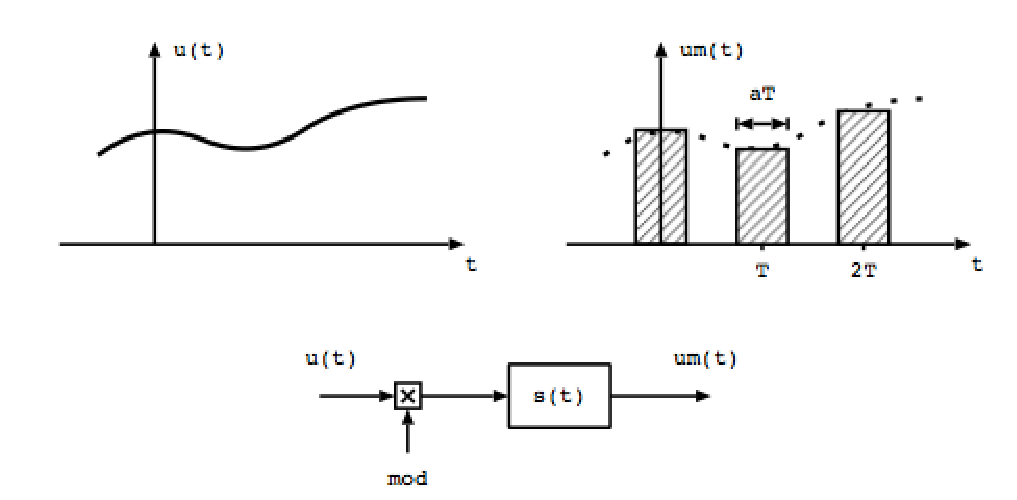
\includegraphics[scale=0.7, trim = 0cm 0cm 0cm 0cm, clip]{./Bilder/PrinzipSignalverbreiterung}
                \caption{Prinzip der Signalverbreiterung}
                \cite{AmplitudenspektrumShap_Top}
        \end{figure}
        
        Auch in diesem Fall ist ein Blick auf das Frequenzspektrum interessant.
        
            \begin{equation*}
                \begin{split}
                    f_m (t) &= [f (t) \cdot \delta_T (t)] \ast \sqcap_{\alpha T} (t)\\
                    F_F (j\omega) &= \left ( \frac{1}{2 \pi} F (j\omega) \ast \omega_T
                    \cdot \delta_T (\omega) \right) \cdot \alpha T \cdot si (\frac{\alpha \omega T}{2})\\
                    &= \alpha \cdot si \left( \frac{\omega \alpha T}{2} \right) \cdot \sum_{k=-\infty}^{\infty} F(j(\omega -
                    k\omega_T))\\
                    &= \alpha \cdot si \left( \frac{\omega \alpha \frac{2 \pi}{\omega_T}}{2} \right) \cdot
                    \sum_{k=-\infty}^{\infty} F(j(\omega - k\omega_T))\\
                    &= \alpha \cdot si \left( \frac{\omega \alpha \pi}{\omega_T} \right) \cdot
                    \sum_{k=-\infty}^{\infty} F(j(\omega - k\omega_T))\\
                \end{split}
            \end{equation*}

        Auch hier erwähnen wir den Sonderfall für das Basisband
        
        \begin{equation*}
        	\begin{split}
        		U_M (j\omega) = \alpha \cdot si \left( \frac{\omega \alpha \pi}{\omega_T}\right) \cdot U (j \omega)
        	\end{split}
        \end{equation*}
        
        Dieses Frequenzspektrum wird nicht nur um den Faktor $\alpha$ gedämpft sondern zusätzlich auch noch um den
        Frequenzabhängigen Faktor $si \left( \frac{\omega \alpha \pi}{\omega_T}\right) $. Diese Dämpfung erscheint auch
        schon in dem Basisfrequenzband und hat eine Verzerrung aller Frequenzbänder zur konsequenz. Das
        Amplitudenspektrum sieht daher folgendermaßen aus:
        
        \begin{figure}[H]
        \centering
            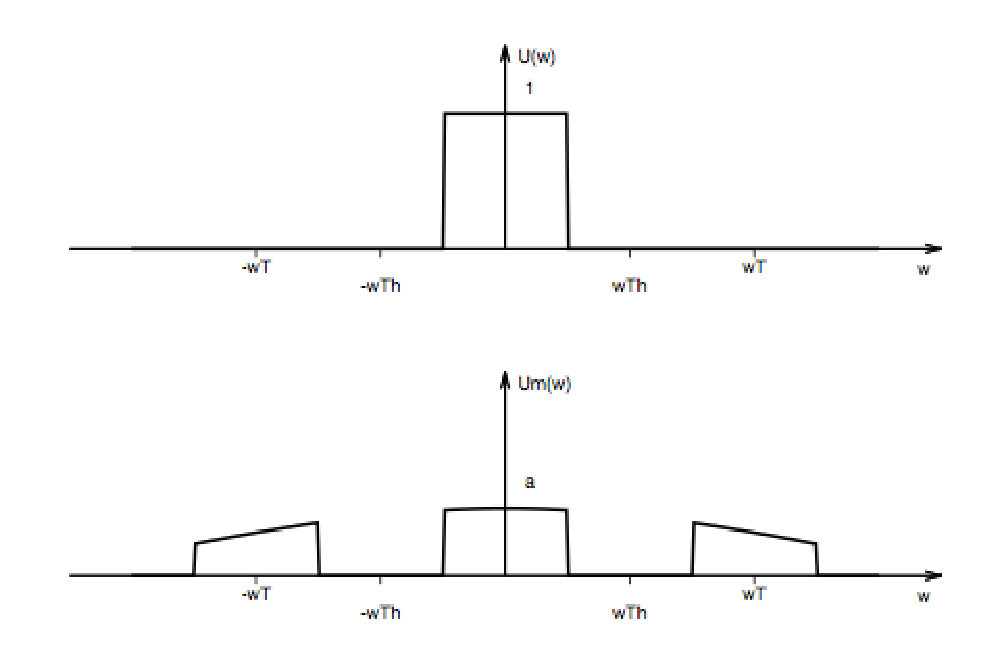
\includegraphics[scale=0.7, trim = 0cm 0cm 0cm 0cm, clip]{AmplitudenspektrumFlat_Top}
                \caption{Amplitudenspektrum Flat-Top}
                \cite{Amplitudenspektrum_Flat_Top}
        \end{figure}
        
        Dieses verzerrte Spektrum lässt sich im Gegensatz zu dem Shape-Top gesampelten Signal nicht durch einen Teifpass
        wieder $100$ prozentig wiederherstellen. Das demodulierte Signal wird weiterhin verzerrt bleiben. Dies ist ein
        Großer Nachteil des Flat-Top sampling.\\
        Der Vorteil dieses Verfahrens ist es, dass das modulierte Signal sich als digitales Signal übertragen lässt und
        sich somit alle weiteren Verfahren der digitalen Übertragungstechnik anwenden lassen. 
    

    	\TODO{Özgü: nocheinmal doie Theorie durchlesen und ggf. umformulieren und ergänzen}
    \end{quote}%subsection
\end{quote}%section

%--------------------------------------------------------------------
%--------------------------------------------------------------------    
\section{Vorbereitungsaufgabe}
\begin{quote}
    \subsection{Herleitung der Spektren}
    \begin{quote}
        Zunächst werden die Formeln für das Spektrum eines abgetasteten Signals
        hergeleitet. Das $\alpha$ steht dabei für das Tastverhältnis.
        
        \subsubsection{Shape-Top-Sampling}
        \begin{quote}
            \begin{equation*}
                \begin{split}
                    f_m (t)   &= f(t) \cdot \sqcap_{\alpha T} (t) \ast \delta_T (t) \\
                    F_S (j\omega) &= \frac{1}{2\pi} F (j\omega) \ast \left [
                    \alpha T \cdot si \left( \frac{\omega \cdot \alpha T}{2} \right) \cdot \omega_T \cdot \delta_{\omega
                    T} (\omega) \right] \\
                    &= \frac{1}{2\pi} F (j\omega) \ast \left [
                    \alpha \frac{2 \pi}{\omega_T} \cdot si \left( \frac{\omega \cdot \alpha T}{2} \right) \cdot \omega_T
                    \cdot \delta_{\omega T} (\omega) \right] \\
                    &= \alpha \cdot F (j \omega) \ast \left ( si \left( \frac{\omega \cdot \alpha T}{2} \right)
                    \sum_{k=-\infty}^{\infty} \delta (\omega - k\omega_T) \right)\\
                    &= \alpha \cdot F (j \omega) \ast \left ( si \left( \frac{\omega \cdot \alpha \frac{2
                    \pi}{\omega_T}}{2} \right) \sum_{k=-\infty}^{\infty} \delta (\omega - k\omega_T) \right)\\
                    &= \alpha \cdot F (j \omega) \ast \left ( si \left( \frac{\omega \cdot \alpha \pi}{\omega_T}
                    \right) \sum_{k=-\infty}^{\infty} \delta (\omega - k\omega_T) \right)\\
                    &= \alpha \cdot F (j \omega) \ast \sum_{k=-\infty}^{\infty} (si(k \pi \alpha) \cdot \delta (\omega -
                    k\omega_T))\\
                    &= \alpha \cdot \sum_{k=-\infty}^{\infty} \left [ si(k \pi \alpha) \cdot F (j(\omega - k\omega_T))
                    \right]\\
                \end{split}
            \end{equation*}
        \end{quote} %ende Subsubsection
        
        \subsubsection{Flat-Top-Sampling}
        \begin{quote}
            \begin{equation*}
                \begin{split}
                    f_m (t) &= [f (t) \cdot \delta_T (t)] \ast \sqcap_{\alpha T} (t)\\
                    F_F (j\omega) &= \left ( \frac{1}{2 \pi} F (j\omega) \ast \omega_T
                    \cdot \delta_T (\omega) \right) \cdot \alpha T \cdot si (\frac{\alpha \omega T}{2})\\
                    &= \alpha \cdot si \left( \frac{\omega \alpha T}{2} \right) \cdot \sum_{k=-\infty}^{\infty} F(j(\omega -
                    k\omega_T))\\
                    &= \alpha \cdot si \left( \frac{\omega \alpha \frac{2 \pi}{\omega_T}}{2} \right) \cdot
                    \sum_{k=-\infty}^{\infty} F(j(\omega - k\omega_T))\\
                    &= \alpha \cdot si \left( \frac{\omega \alpha \pi}{\omega_T} \right) \cdot
                    \sum_{k=-\infty}^{\infty} F(j(\omega - k\omega_T))\\
                \end{split}
            \end{equation*}
        \end{quote} %ende Subsubsection
    \end{quote}  % Ende Subsection        
    \subsection{Skizzieren}
    \begin{quote}
                
        Danach werden die resultierenden Spektren $F_S (j\omega)$ und $F_F (j\omega)$
        für das Nutzsignal
        \begin{equation*}
        f(t) = A \cdot cos(\frac{\omega_T}{5}t)     
        \end{equation*}
		    mit $\alpha = 0.5$ und $\omega_T = 20\pi kHz$.
        
        
         \begin{figure}[H]
            \centering
                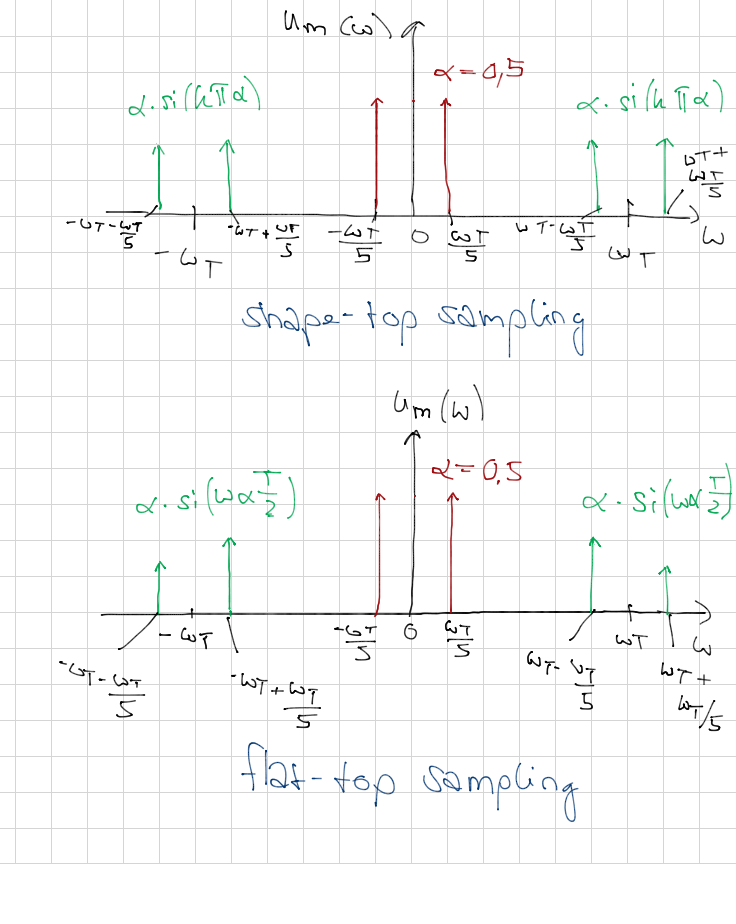
\includegraphics[scale=0.3, trim = 0cm 0cm 0cm 0cm,
                clip]{./Bilder/vorbereitungsskizze}
                    \caption{Skizze}
        \end{figure}
        
        Es ist zu sehen, dass sich die Amplituden der Spektren mit einem
        Si-Funktionsfaktor, welcher von dem eingesetzten $\alpha$ abhängt, verringern.
        Bei der shape-top Abtastung ist dieser Faktor unabhängig von der Frequenz
        $\omega$. Daher sind die Amplituden der Peaks, die an den Grenzen eines
        Frequenzbandes entstehen, immer gleich groß.        
        Bei der flat-top Abtastung ist dieser Faktor sogar von der Frequenz abhängig, daher entsteht 
        eine Amplitudenverringerung von zwei Peaks an den Rändern eines
        Frequenzbandes.\\
        Mit $\alpha$ gegen $0$ geht auch die Amplitude des Basisbands (k = $0$) gegen
        $0$. Somit werden alle folgenden Peakamplituden (deren Amplituden sich bei der
        shape-top Abtastung mit $\alpha \cdot si(k \pi \alpha)$ und bei der flat-top
        Abtastung mit $\alpha \cdot si(\frac{\omega \alpha T}{2})$ bilden) ebenfalls
        verschwindend gering. ist das $\alpha$ aber $1$, beträgt die Amplitude des
        Basisbands $1$ und die folgenden Peakamplituden lassen sich wie bereits
        erwähnt berechnen.
        
        \TODO{Ist das okay so Boris?}
        
    \end{quote}  % Ende Subsection    
    
    \subsection{Planung und Durchführung}
    \begin{quote}
        Außerdem wird die Planung zur Praktikumsdurchführung im voraus gemacht. Für
        den Versuch haben wir uns folgendes überlegt.\\
        \TODO{hier die Skizze}
        
        Zuerst müssen die Quellsignale moduliert werden. Das Sinussignal
        kommt direkt aus der Quelle auf dem Steckbrett mit $2 kHz$ Fequenz und
        $2V$ Amplitude. An diesem Signal wird nichts verändert. Beim
        Rechtecksignal beträgt die Amplitude der Quelle auf dem Steckbrett $5V$, daher 
        muss das Signal zunächst in einen Verstärker/Dämpfer geführt werden.
        Dazu verwenden wir den Addierer mit dem integrierten Dämpfer und
        reduzieren das Signal von $5V$ zuerst mit dem Faktor $\frac{4}{5}$ auf $4V$ und addieren dann $-2V$ drauf, um
        ein bipolares Rechtecksignal mit einer Peak-to-Peak Amplitude von $-2V$
        bis $+2V$ zu erhalten.\\
        Nun müssen diese Signale abgetastet werden:
        
        Für das shape-top sampling wird das Sinus-Quellsignal in den
        Schalter geführt, welcher über das Rechteck-Tastsignal mit $5V$ Amplitude und $10 kHz$ bzw. $20 kHz$
        Abtastfrequenz zustandsgesteuert ist. Durch den Schalter wird der Sinus
        entsprechend abgetastet und kann mithilfe des PicoScope grafisch
        dargestellt werden.\\ 
        Das modulierte Rechteckquellsignal wird ebenfalls in den
        zustandgesteuerten Schlater geführt, wo es dann durch shape-top sampling
        abgetastet wird. 
        
        \vspace{0.5em}
        
        Für das flat-top sampling wird zusätzlich ein Sample and Hold Glied
        verwendet. Dieser befindet sich auf dem Steckbrett direkt über dem
        verwendeten Schalter und ist ebenfalls über das Rechtecktastsignal
        gesteuert. Beide Quellsignale werden hierbei zunächst in das Sample and
        Hold Glied geführt und aus dessen Ausgang in den Schalter
        weitergeleitet. So wird erst die zum Abtastzeitpunkt vorhandene
        Amplitude ermittelt und danach die Abtastung vollzogen. Das enstandene
        Signal kann anhand PicoScope grafisch mit dem Quellsignal ins Vergleich gesetzt
        werden.
        
        
        \TODO{Blockschaltbilder einfügen (mit iPad)}
               
    \end{quote}  % Ende Subsection	
    
    \subsection{Matlab-Simulation}
    \begin{quote}
        Zuletzt wird eine MATLAB-Simulation der Abtastung mittels Signalausblendung
        und Signalverbreiterung für ein Sinussignal als Quellsignal und der
        Abtastfrequenz von $400 kHz$ ausgeführt. Das verwendete Quellsignal
        hatte eine Amplitude von $2V$ und eine Frequenz von $2 kHz$. Das
        Abtastrechtecksignal hatte eine variable Frequenz ($10 kHz und 20 kHz$),
        eine variable Amplitude (gewählt haben wir $1V, 2V$ und $3V$) und ein
        variables Tastverhältnis von $0.2, 0.5$ oder $0.7$.\\
        Für den hiesigen Vergleich haben wir nur die Abtastamplituden $1V$ udn $3V$
        verwendet.
        
        Zuerst betrachten wir die Simmulationsergebnisse der Abtastung durch
        Signalausblendung:
        
         \begin{figure}[H]
        \centering
        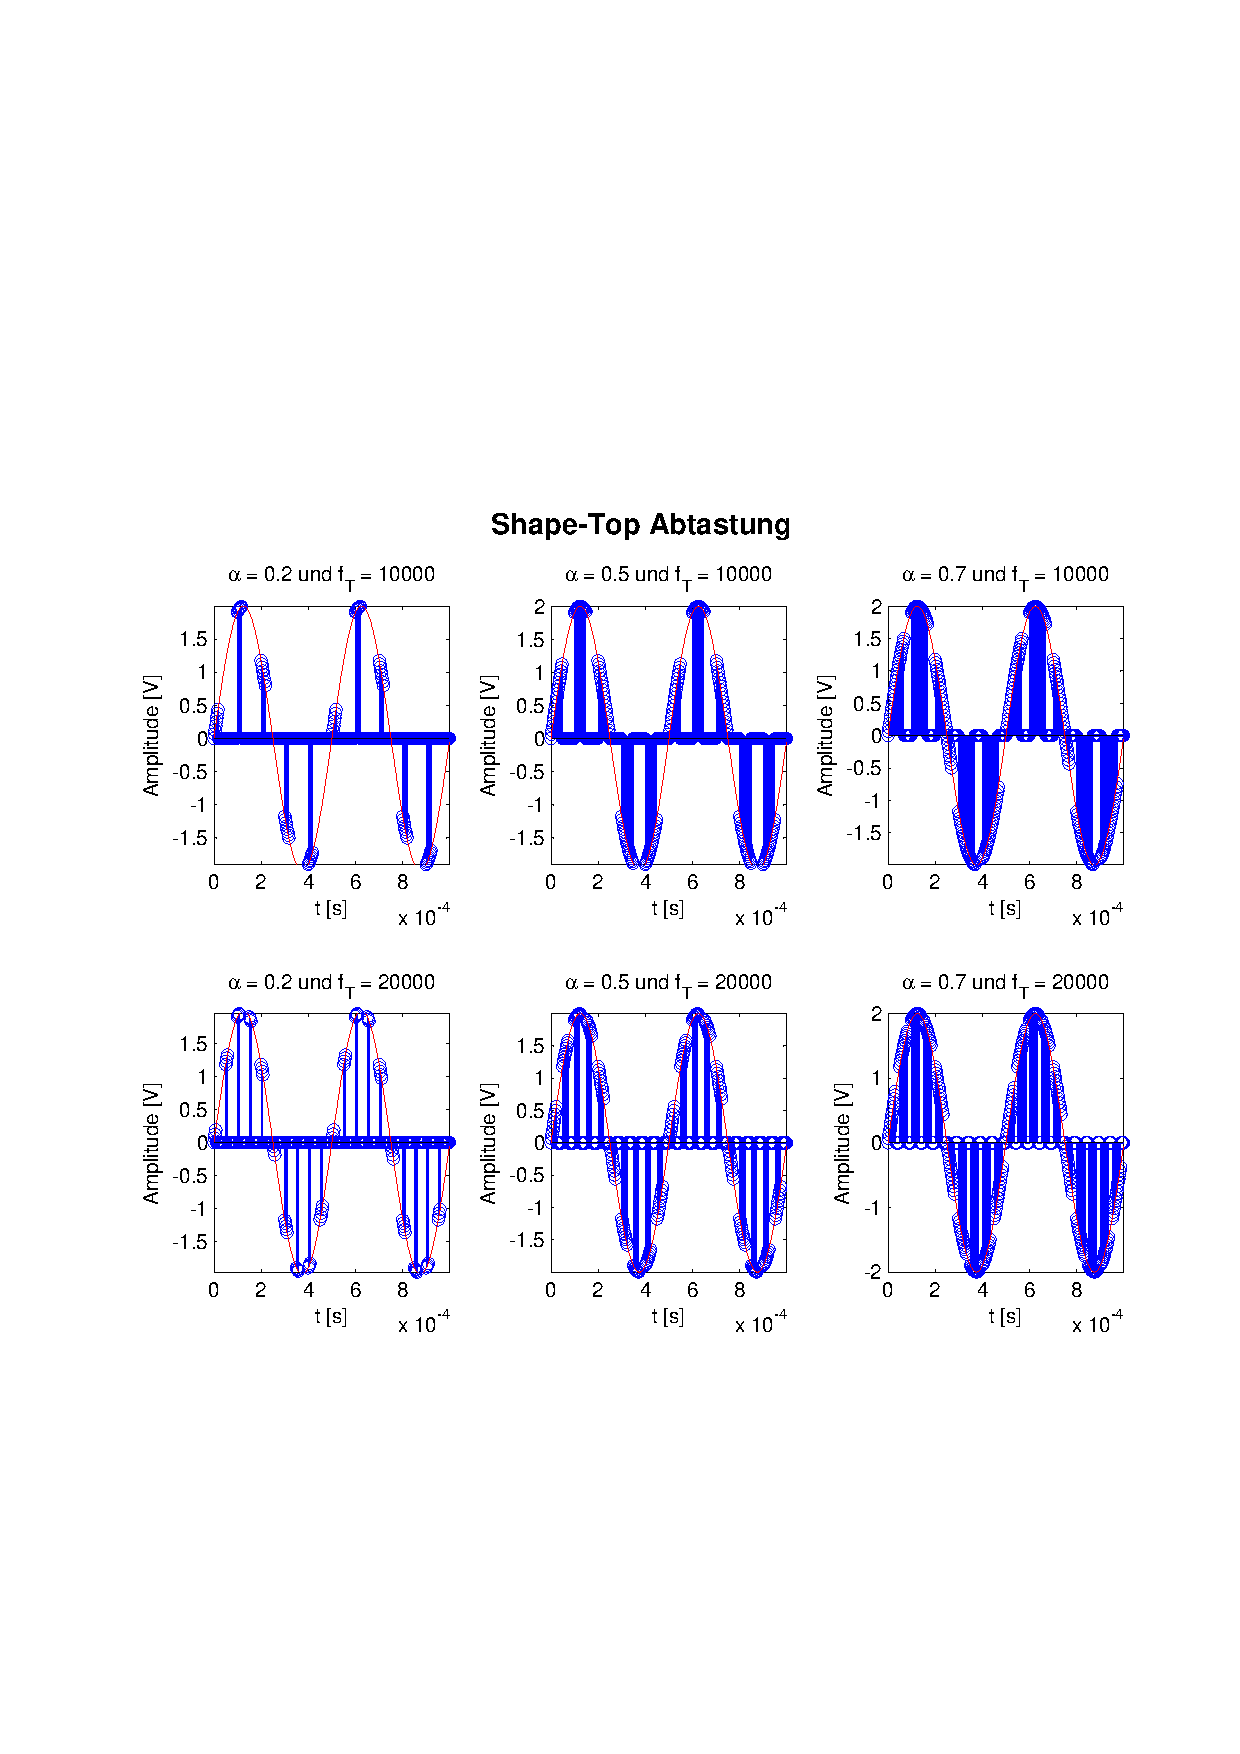
\includegraphics[scale=0.7, trim = 1.5cm 6cm 1cm 8cm,
        clip]{./Bilder/shape-top-zeit_1V}
            \caption{Zeitsignal mit shape-top-sampling und Abtastamplitude 1V}
  	    \end{figure}
  	    
  	    
  	    \begin{figure}[H]
    \centering
        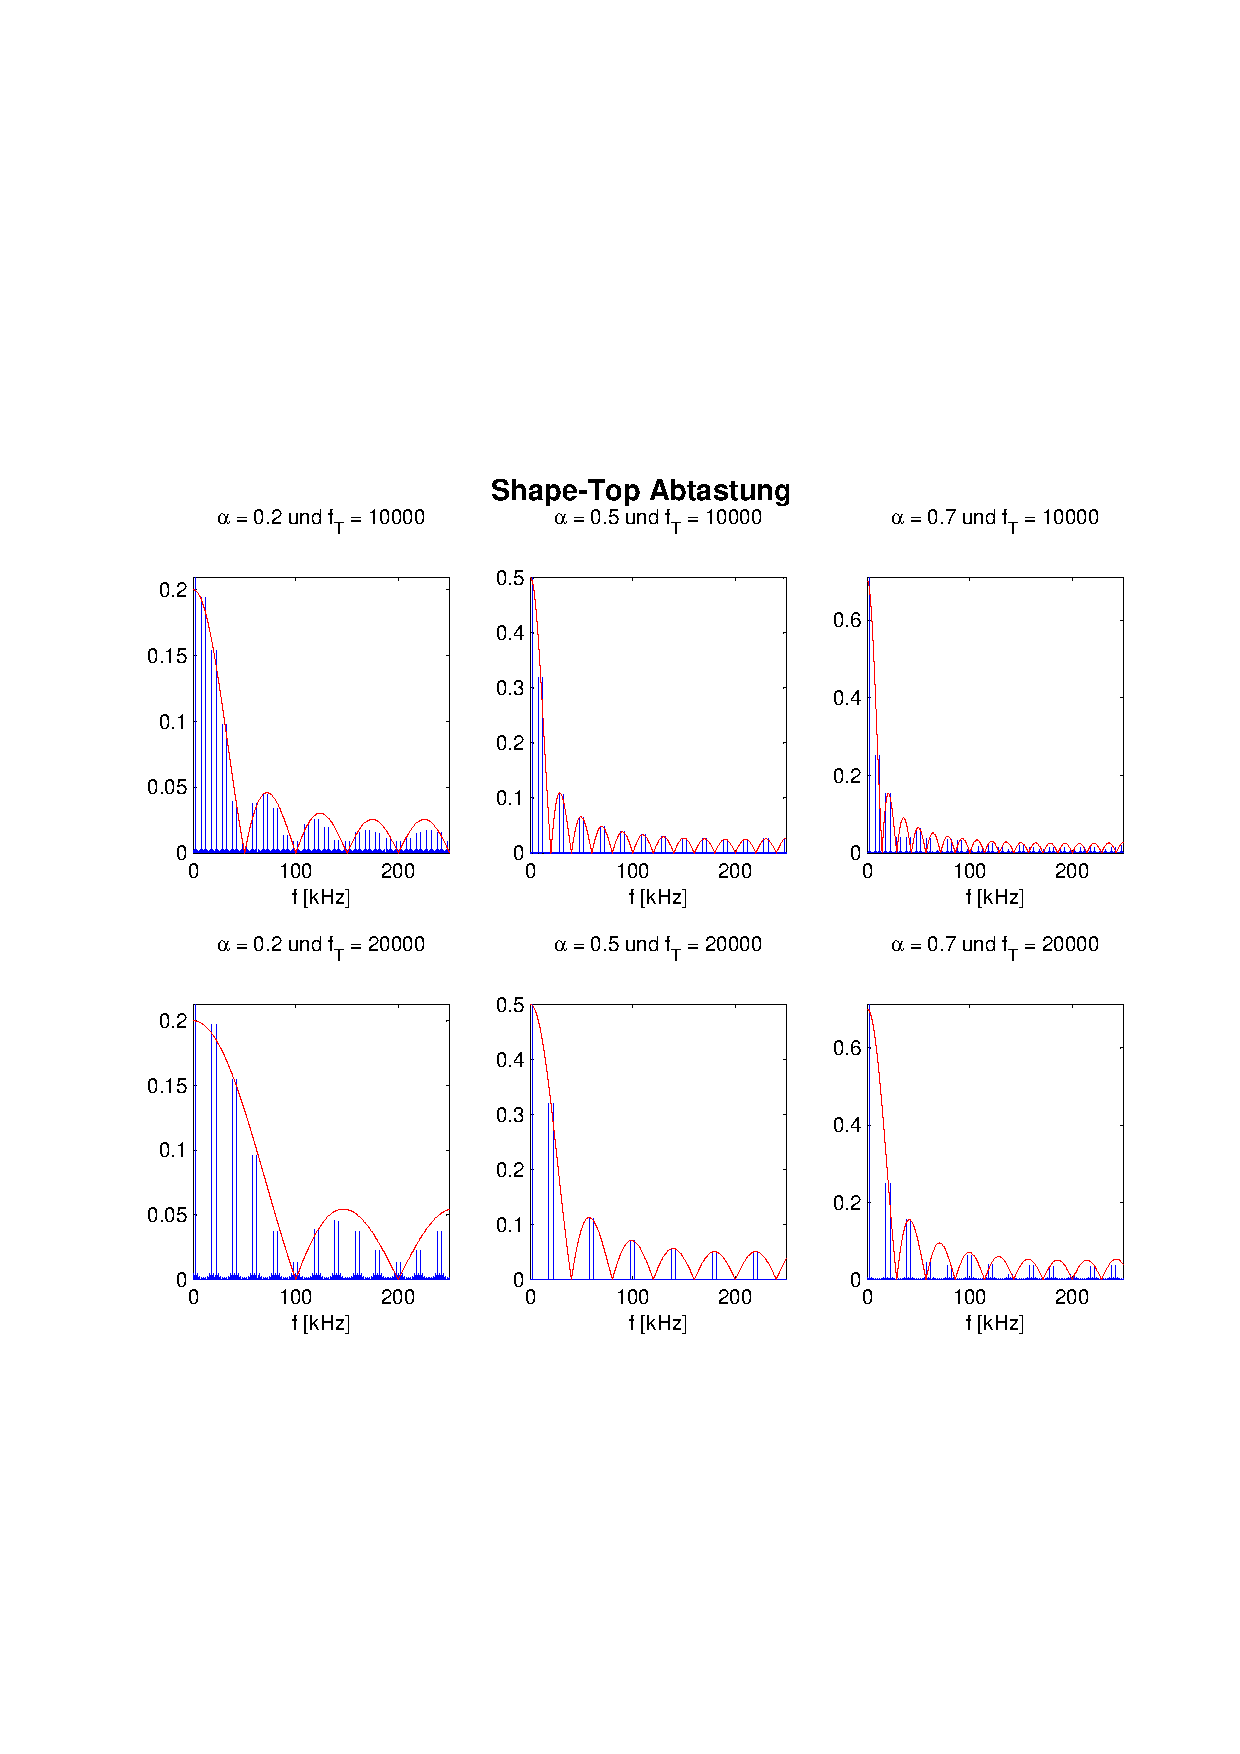
\includegraphics[scale=0.7, trim = 0cm 0cm 0cm 0cm,
        clip]{./Bilder/shape-top-freq_1V}
            \caption{Frequenzsignal mit shape-top-sampling und Abtastamplitude
            1V}
  	    \end{figure}
  	    
  	    Im Zeitsignal sieht man eine maximale Amplitude von $2V$, welche durch
  	    die Multiplikation von den $2V$ des Quellsignals und dem $1V$ des
  	    Abtastsignals entsteht. Die Form der Rechtecke nehmen oben den
  	    Sinusverlauf des Quellsignals an, was im Zeitsignal den Unterschied zu
  	    der flat-top Abtastung ausmacht. Zusätzlich kann man deutlich sehen, dass
  	    die Verdopplung der Abtastfrequenz ungefähr doppelt so viele abgetastete Stellen ergibt und 
  	    dass ein größeres Tastverhältnis die Breite der Dauer der Abtastung erhöht. 
  	    Als Umhüllende haben wir das Quellsignal verwendet.\\
  	    Im simmulierten Spektrum kann man erkennen, dass die Amplituden der
  	    drei Basisbänder für die drei Tastverhältnisse exakt dem eingesetzten
  	    Tastverhältnis $\alpha$ mal $1V$ entsprechen. Mit wachsender Frequenz
  	    nehmen die Peaks deutlich an Amplitude ab. Außerdem kann man sehen, dass
  	    die auftretenden Peakpaare immer die gleiche Amplitude besitzen. Dieses
  	    unverzerrte Spektrum war bei einer shape-top Abtastung zu erwarten.
  	    Die Umhüllende des Spektrums ist eine Si-Funktion.
  	    
    	Wenn man nun die Amplitude des Abtastsignals erhöht, erhält man folgende
    	Plots:
    	
    	\begin{figure}[H]
    \centering
        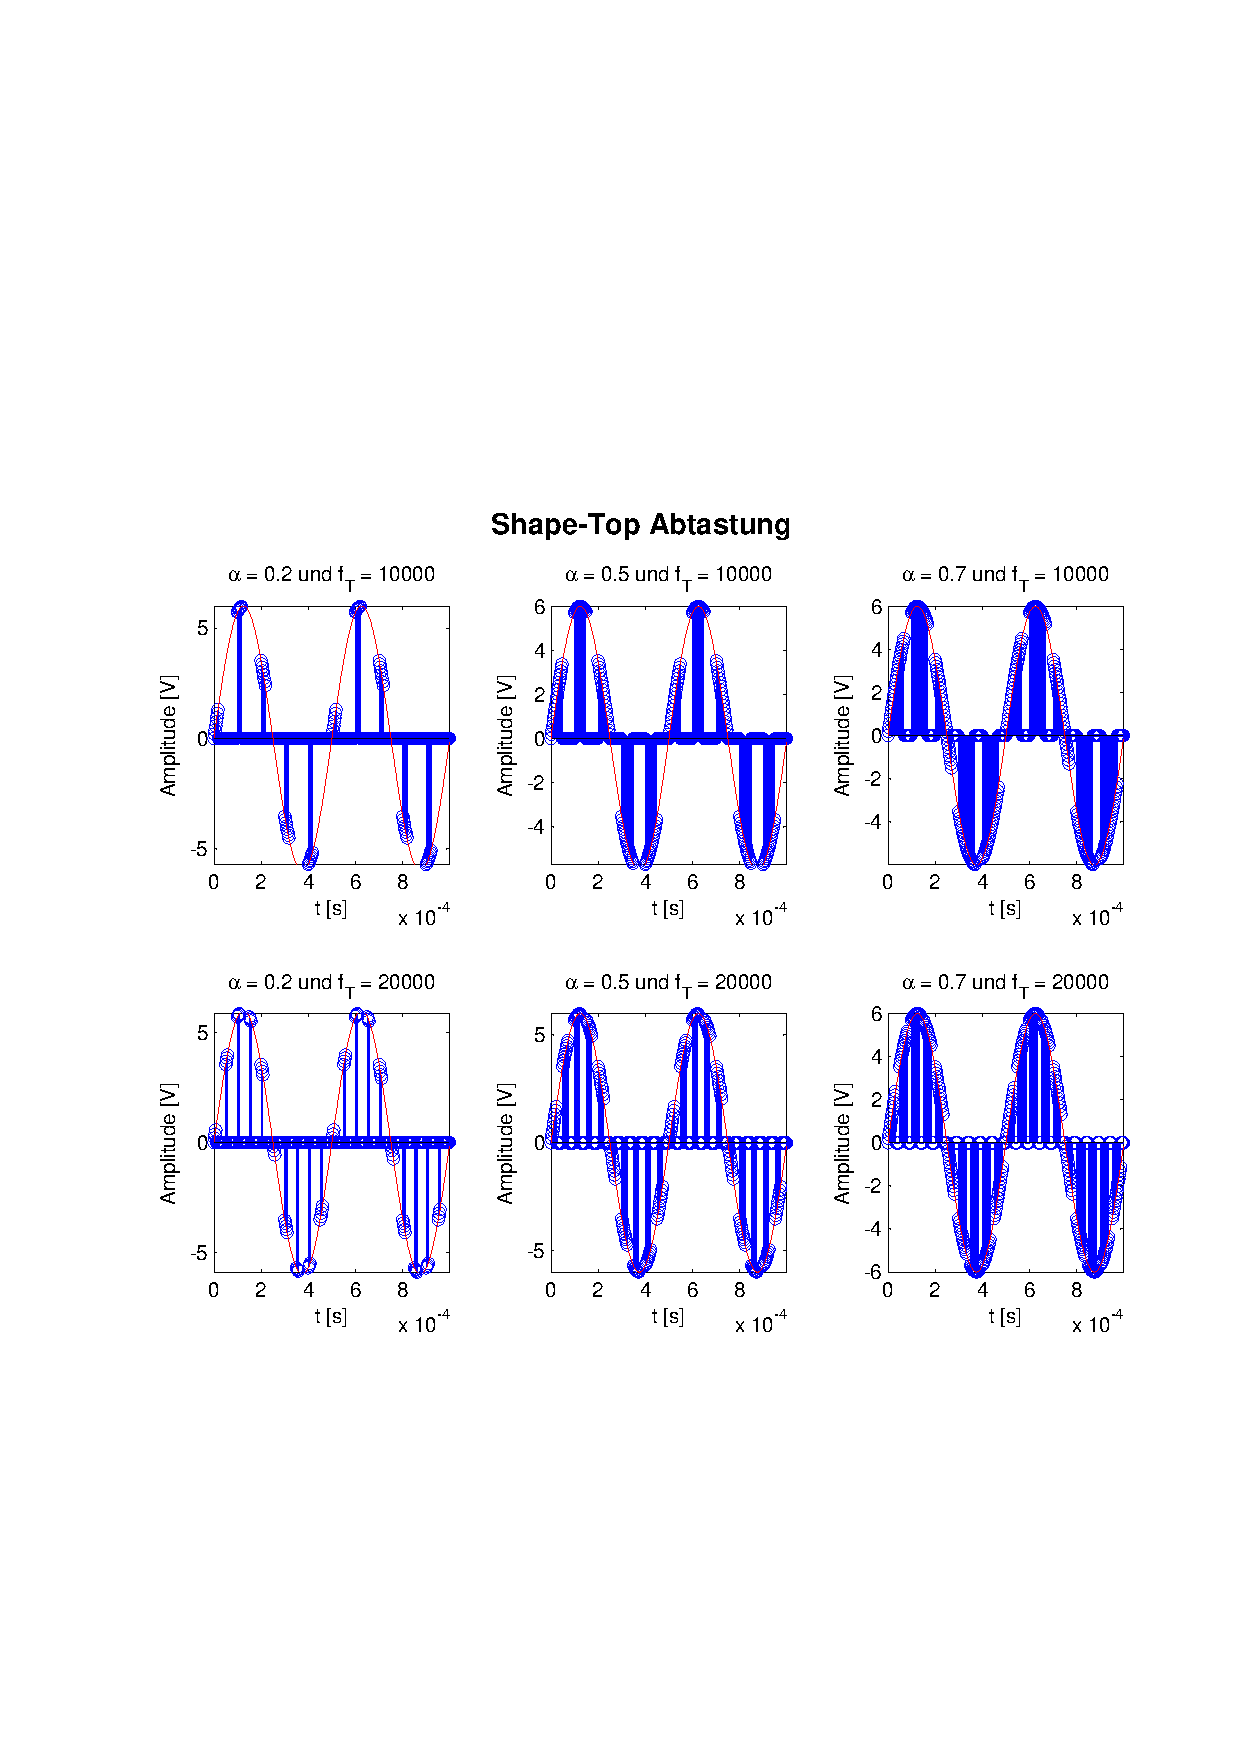
\includegraphics[scale=0.7, trim = 0cm 0cm 0cm 0cm,
        clip]{./Bilder/shape-top-zeit_3V}
            \caption{Zeitsignal mit shape-top-sampling und Abtastamplitude 3V}
  	    \end{figure}
  	    
  	    
  	    \begin{figure}[H]
    \centering
        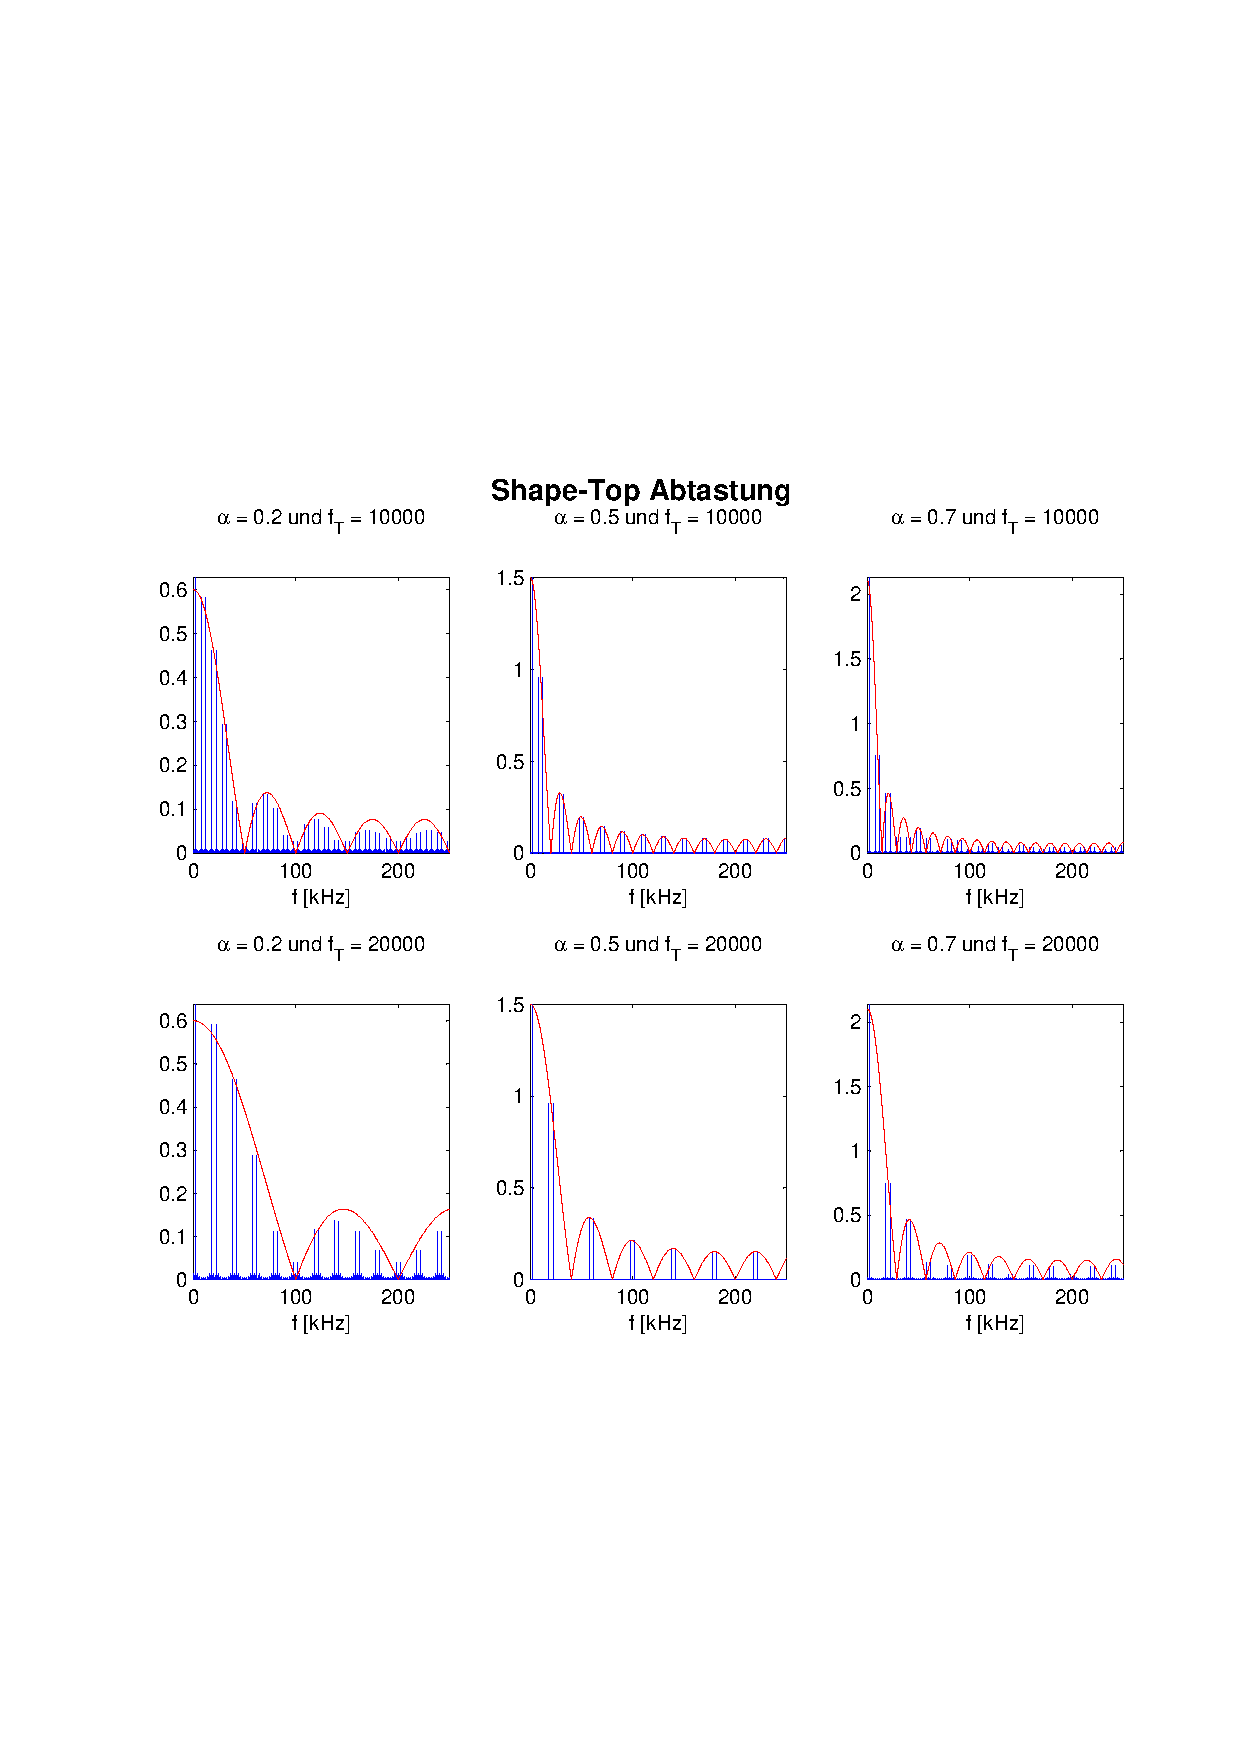
\includegraphics[scale=0.7, trim = 0cm 0cm 0cm 0cm,
        clip]{./Bilder/shape-top-freq_3V}
            \caption{Frequenzsignal mit shape-top-sampling und Abtastamplitude
            3V}
  	    \end{figure}
  	    
  	    
  	    Im Zeitsignal beträgt die Amplitude diesmal $6V$, welche durch die
  	    Multiplikation von $2V \cdot 3V$ entsteht. Alle anderen Auswirkungen der
  	    Tastfrequenz und des Tastverhältnisses bleiben gleich.\\
  	    Auch im Spektrum liegt der einzige Unterschied in den Maximalamplituden,
  	    welche nun um den Faktor $3$ (durch die $3V$ Amplitude des Abtastsignals)
  	    größer sind.
  	    
  	    \vspace{1em}
  	    
  	    Nun betrachten wir die Simmulationsergebnisse der Abtastung mit
  	    Signalverbreiterung:
  	    
  	    \begin{figure}[H]
    \centering
        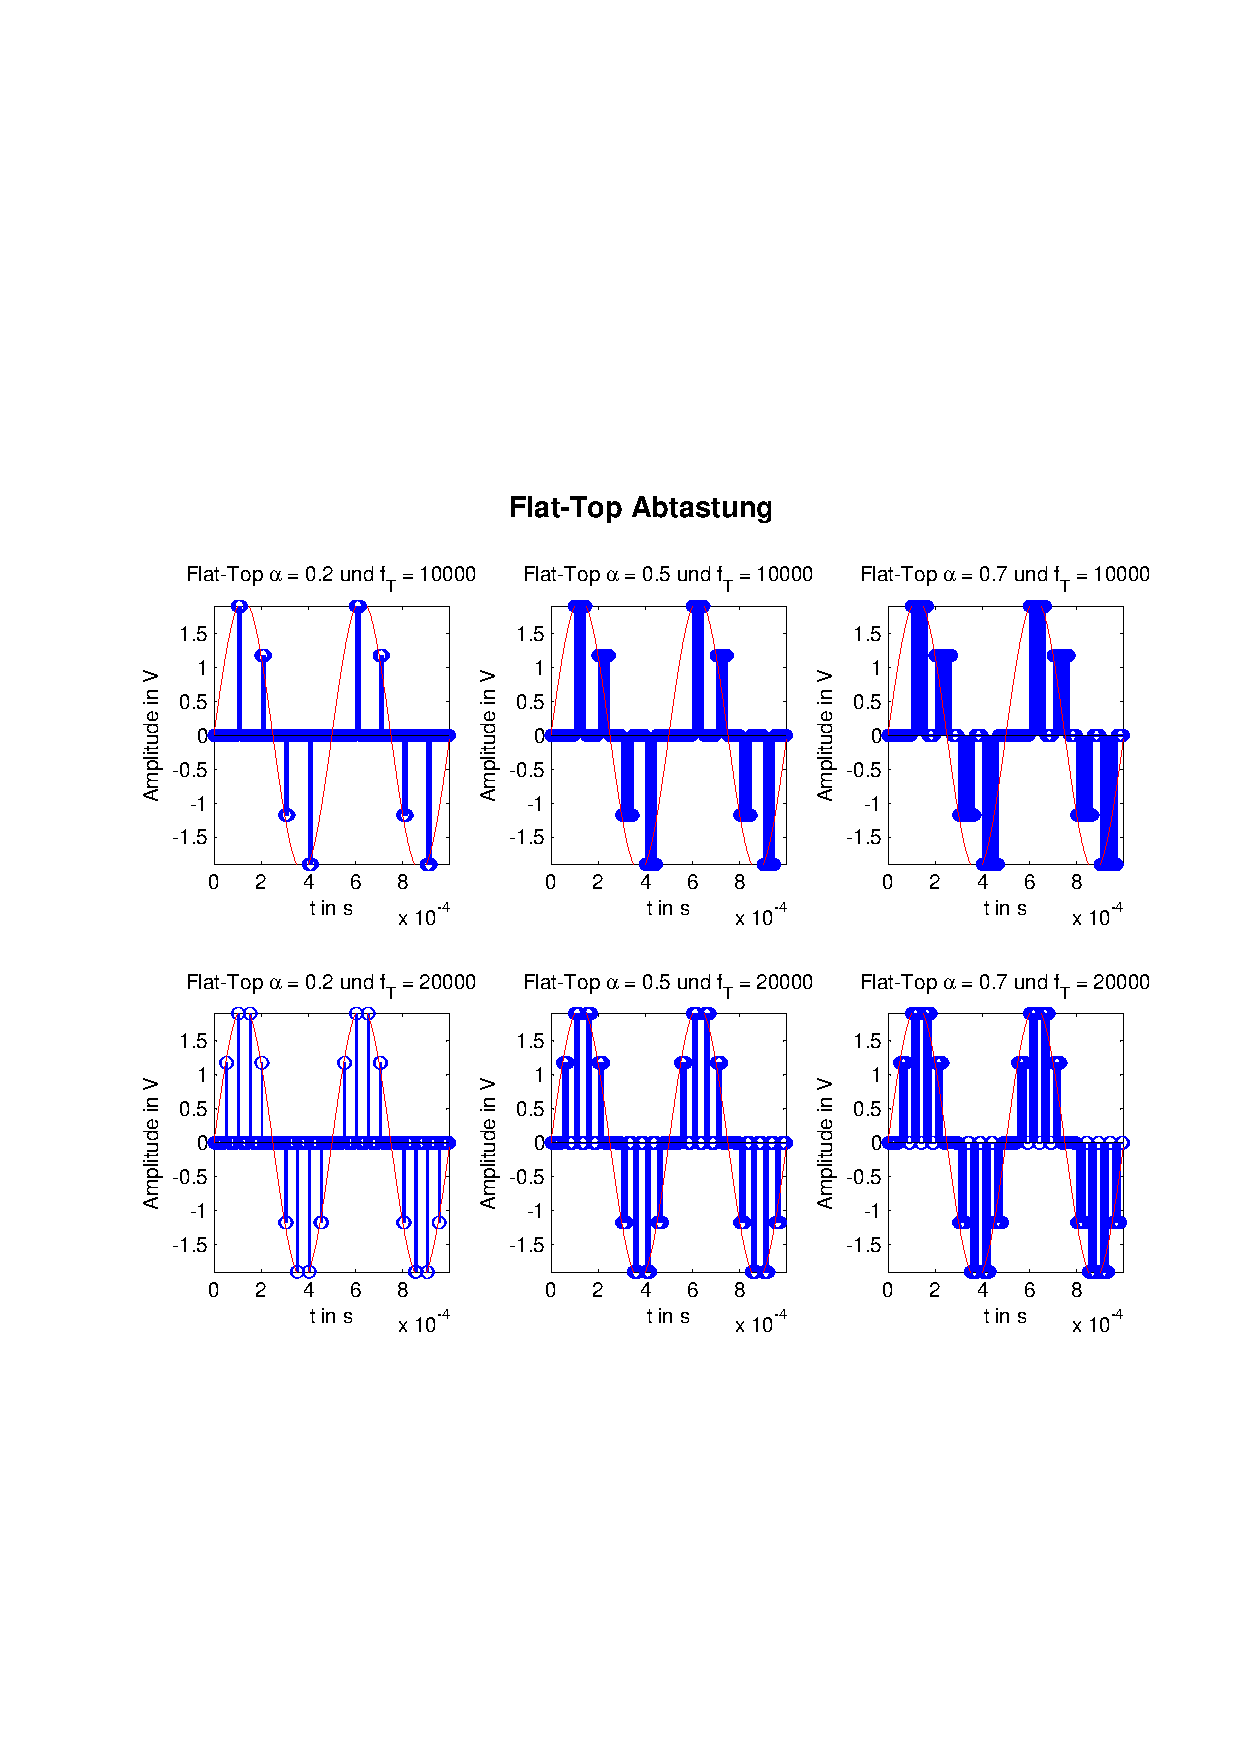
\includegraphics[scale=0.7, trim = 0cm 0cm 0cm 0cm,
        clip]{./Bilder/flat-top-zeit_1V}
            \caption{Zeitsignal mit flat-top-sampling und Abtastamplitude 1V}
  	    \end{figure}
  	    
  	    
  	    \begin{figure}[H]
    \centering
        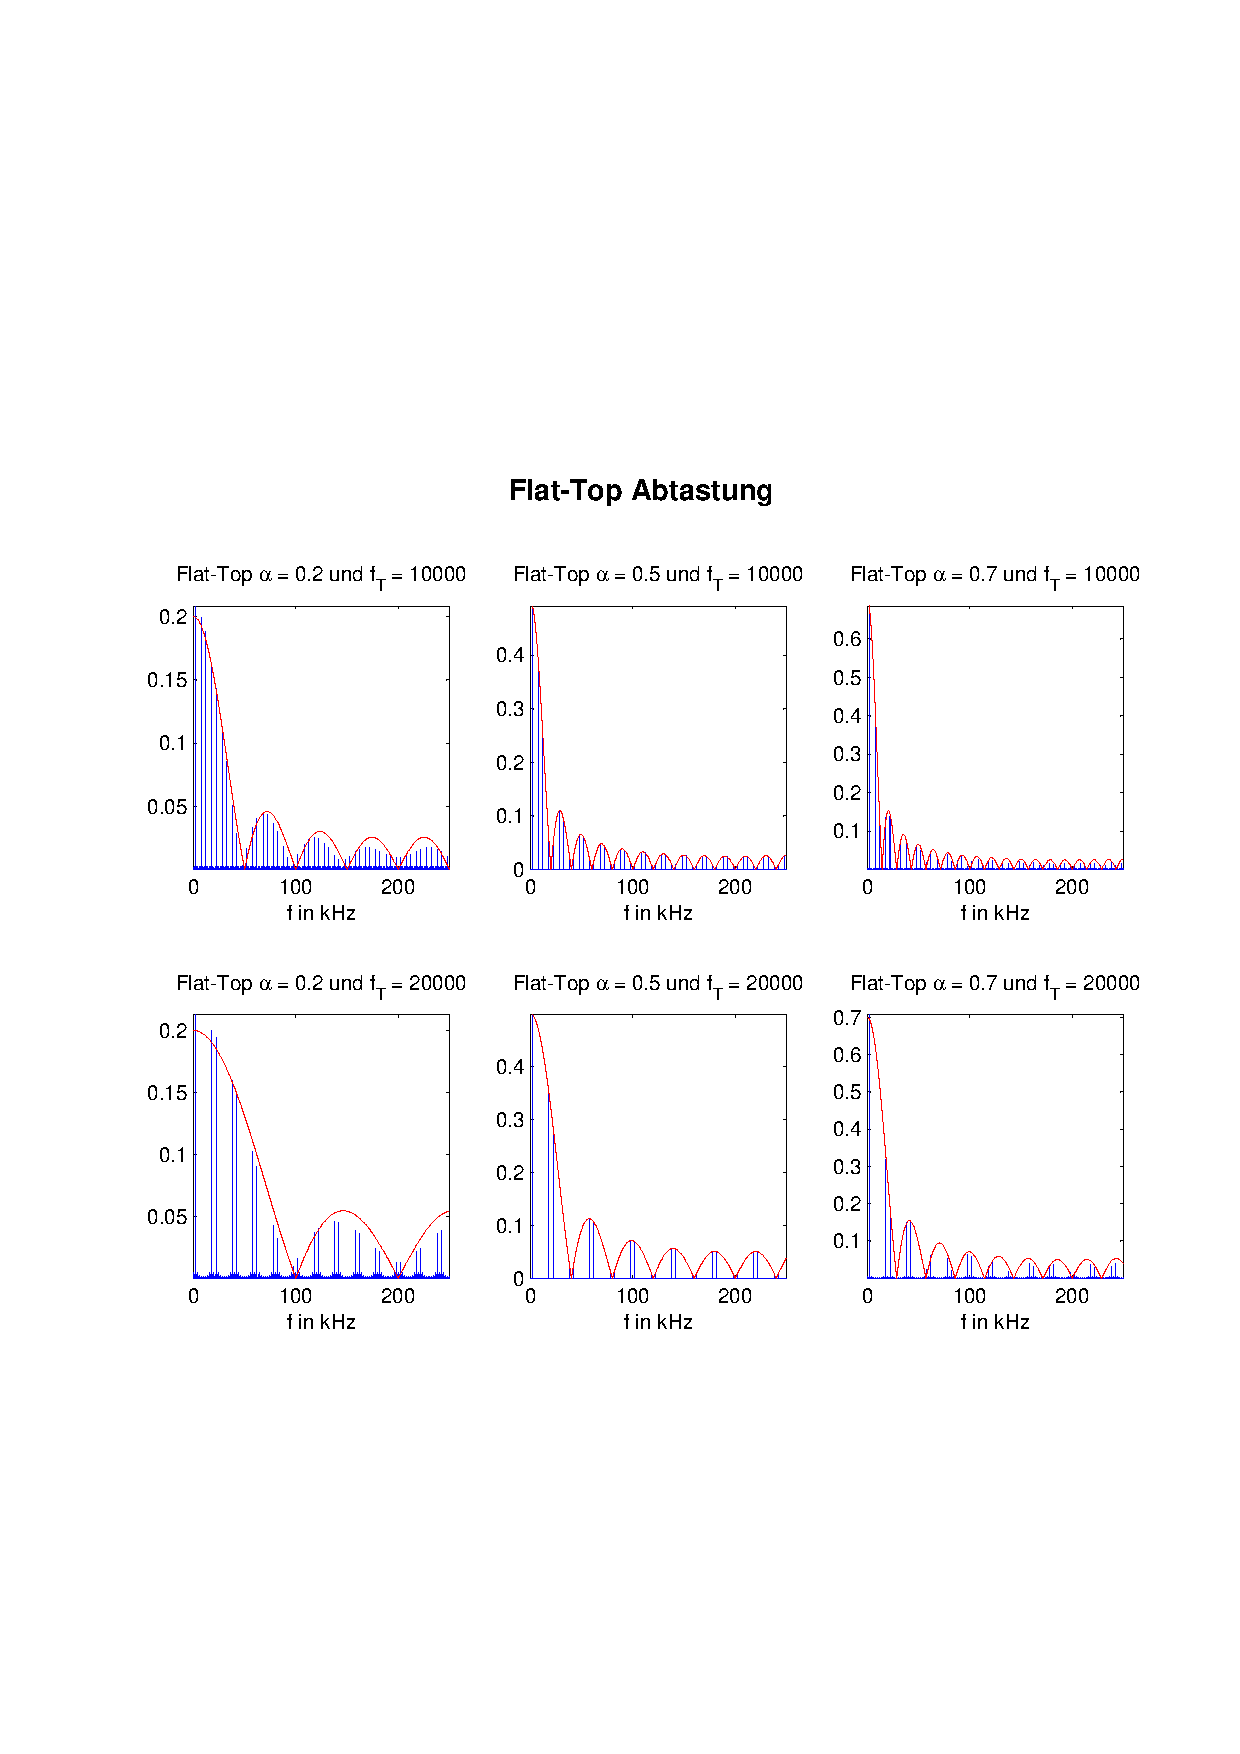
\includegraphics[scale=0.7, trim = 0cm 0cm 0cm 0cm,
        clip]{./Bilder/flat-top-freq_1V}
            \caption{Frequenzsignal mit shape-top-sampling und Abtastamplitude
            1V}
  	    \end{figure}
  	    
  	    Die Amplituden, die Breiten und die Häufigkeiten der abgetasteten Stellen
  	    stimmen bei der flat-top Abtastung mit den Werten des Zeitsignals der
  	    shape-top Abtastung überein. Der einzige Unterschied, den man wie erwartet sehen
  	    kann, ist, dass die Rechtecke sich nicht dem Sinusverlauf anpassen
  	    sondern ab der Abtaststelle die Sinusamplitude annehmen und durch das
  	    Hold-Glied über die Dauer der Abtastung behalten. Daher sind diese
  	    Rechtecke oben flach.\\
  	    Durch die DFT dieser Rechtecke aus dem Zeitsignal entstehen in dem
  	    Spektrum Peaks mit frequenzabhängiger Amplitude, die deutlich
  	    besser in die umhüllende Si-Funktion passen, als das Spektrum einer
  	    shape-top Abtastung. Ansonsten verhält sich das Spektrum im Bezug auf
  	    Tastfrequenz und -verhältnis nicht anders als bei der Abtastung durch
  	    Signalausblendung.
  	    
  	    Nun wird wieder die Abtastamplitude erhöht:
        
        
        \begin{figure}[H]
        \centering
            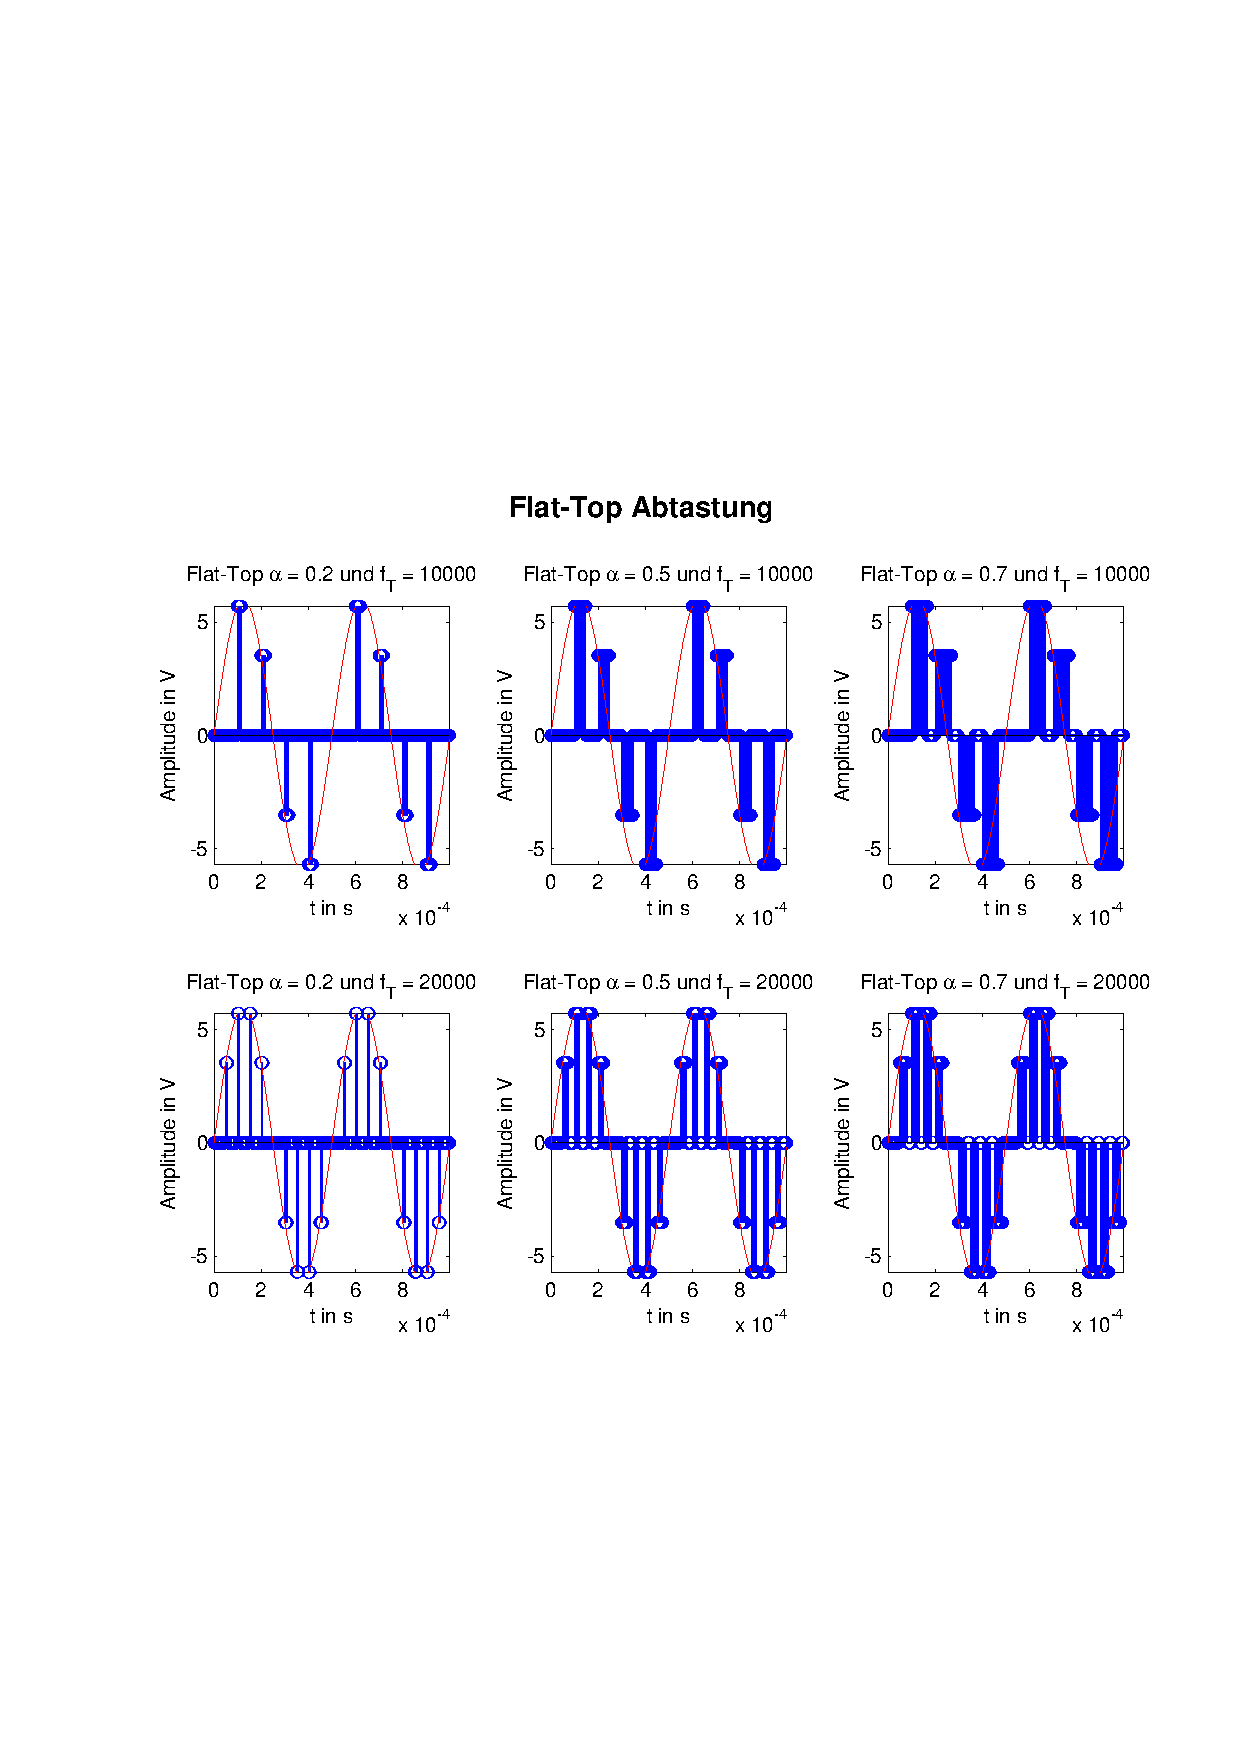
\includegraphics[scale=0.7, trim = 1.5cm 6cm 1cm 8cm,
            clip]{./Bilder/flat-top-zeit_3V}
                \caption{Zeitsignal mit flat-top-sampling und Abtastamplitude 3V}
        \end{figure}
        
        
        \begin{figure}[H]
        \centering
            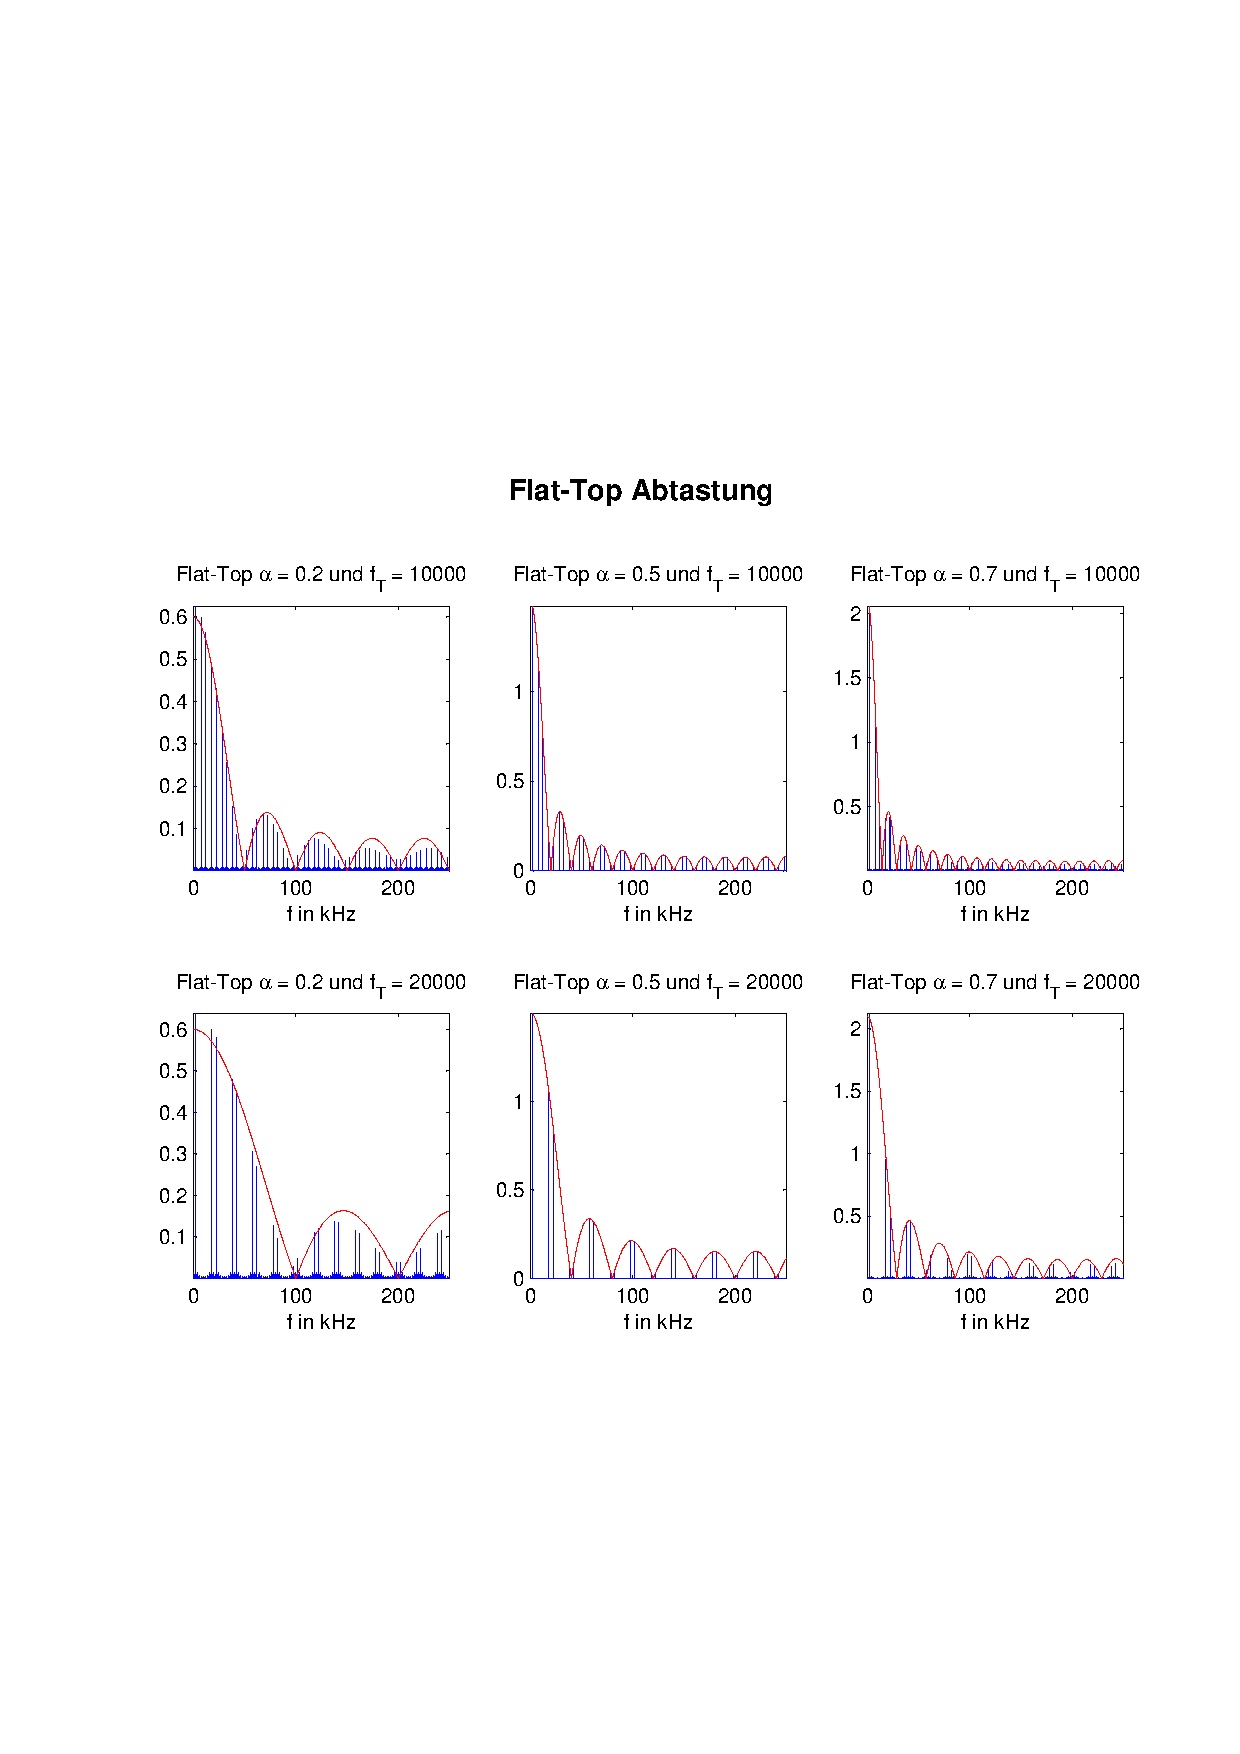
\includegraphics[scale=0.7, trim = 1.5cm 6cm 1cm 8cm,
            clip]{./Bilder/flat-top-freq_3V}
                \caption{Frequenzsignal mit flat-top-sampling und Abtastamplitude
                3V}
        \end{figure}
        
        
        Die Amplituden im Zeitsignal betragen wieder $6V$ und die Amplituden der
        Basisbänder nehmen die Werte $3V \cdot \alpha$ an. Ansonsten ist das
        Spektrum erneut deutlich verzerrter und alle anderen erwarteten
        Ergebnisse können auch hier wahrgenommen werden. 
        
    \end{quote}  % Ende Subsection	


\end{quote}%Theorie beenden

%--------------------------------------------------------------------
%--------------------------------------------------------------------    

    
    \section{Labordurchführung}
    \begin{quote}
         
         Nachdem wir die beiden realisierbaren, nichtidealen Abtastverfahren
         theoretisch realisiert haben, wurde nun die praktische Untersuchung
         dieser Verfahren Pulsamplitudenmodulation zur Diskretisierung von
         zeitkontunierlichen Signalen durchgeführt. Dazu wurde, je nachdem
         welches Abtastverfahren untersucht werden sollte, eine
         Pulsamplitudenmodulationstrecke mit verschiedenen variablen Parametern
         entworfen und anhand dieser Strecke die Zeitsignale und die daraus
         entstehenden Spektren betrachtet.\\
         
         Als Abtastsignal verwendeten wir ein unipolares Rechtecksignal mit $5V$
         Amplitude und einer Abtastfreuquenz von entweder $10 kHz$ oder $20
         kHz$. Das Tastverhältnis wurde bei den Messungen zwischen $0.2$, $0.5$
         und $0.7$ abgewechselt. Dieses Abtastsignal erzeugten wir mithilfe des
         Signalgenerator und kontrollierten es vor jeder Messung mit dem
         Oszilloskop.\\
         
         Als Quellsignale wurden ein Sinus- und ein Rechtecksignal, sowie ein
         Rechtecksignal mit vorheriger RC-Tiefpassfilterung eingesetzt. Für den
         Sinus verwendeten wir die Quelle auf dem Steckbrett, welcher uns, wie
         bereits in der Vorbereitungsaufgabe zum Versuchsaufbau erklärt, eine
         Amplitude von $2V$ und eine Frequenz von $2 kHz$ zur Verfügung stellte. 
         Die Einrichtung des Rechteckquellsignals war etwas aufwendiger. Da das
         Steckbrett tatsächlich nur einen unipolaren Rechteck mit der Amplitude
         von $5V$ liefert, musste es erst auf das erwünschte bipolare Rechteck
         mit der Peak-to-Peak Spannung von $4V$ umgestellt werden.
         
         
   	\end{quote}%beende Labordurchführung

%--------------------------------------------------------------------
%--------------------------------------------------------------------    
    	    
    
    \section{praktische Umsetzung}
    \begin{quote}
    Die praktische Umsetzung des Versuchs ist für beide Abtastverfahren gleich.
    
    \TODO{zu Ende bringen}
    \end{quote}%beende praktische Umsetzung
    
%--------------------------------------------------------------------
%--------------------------------------------------------------------    

    
    \section{Auswertung}
    \begin{quote}    
        \TODO{Auswertung schreiben}
    \end{quote}%beende Auswertung
    
    \section{Zusammenfassung}
    \begin{quote}
    	\TODO{Zusammenfassung schreiben}
    \end{quote}%beende Zusammenfassung
         

\TODO{Boris: öfter mal ein Überraschungsgeschenk für deine beste Freundin
besorgen!!}

%--------------------------------------------------------------------
%--------------------------------------------------------------------    


\begin{thebibliography}{999}
 \bibitem {PrinzipSignalausblendung} Prof. Dr.-Ing. Sikora, Thomas; Prof. Dr.-Ing. Noll, Peter: Einführung in die
 Nachrichtenübertragung, S.257
\bibitem {AmplitudenspektrumShap_Top} Prof. Dr.-Ing. Sikora, Thomas; Prof. Dr.-Ing. Noll, Peter: Einführung in die
 Nachrichtenübertragung, S.258
\bibitem {Amplitudenspektrum_Flat_Top} Prof. Dr.-Ing. Sikora, Thomas; Prof. Dr.-Ing. Noll, Peter: Einführung in die
 Nachrichtenübertragung, S.259
 



%Name, Vorname.; evtl. Name2, Vorname2.: Titel des Dokumentes
%oder Buches, Zeitschrift/Verlag/URL (Auflage, Erscheinungsort, -jahr), ggf. Seitenzahlen
% \bibitem {PasevalscheTheorem} \url{https://de.wikipedia.org/wiki/Parsevalsches_Theorem}, Zugriff
% 23.05.2012
\end{thebibliography}

\end{document}
  	    
  	    Nun wird wieder die Abtastamplitude erhöht:
  	    
  	    
  	    \begin{figure}[H]
    \centering
        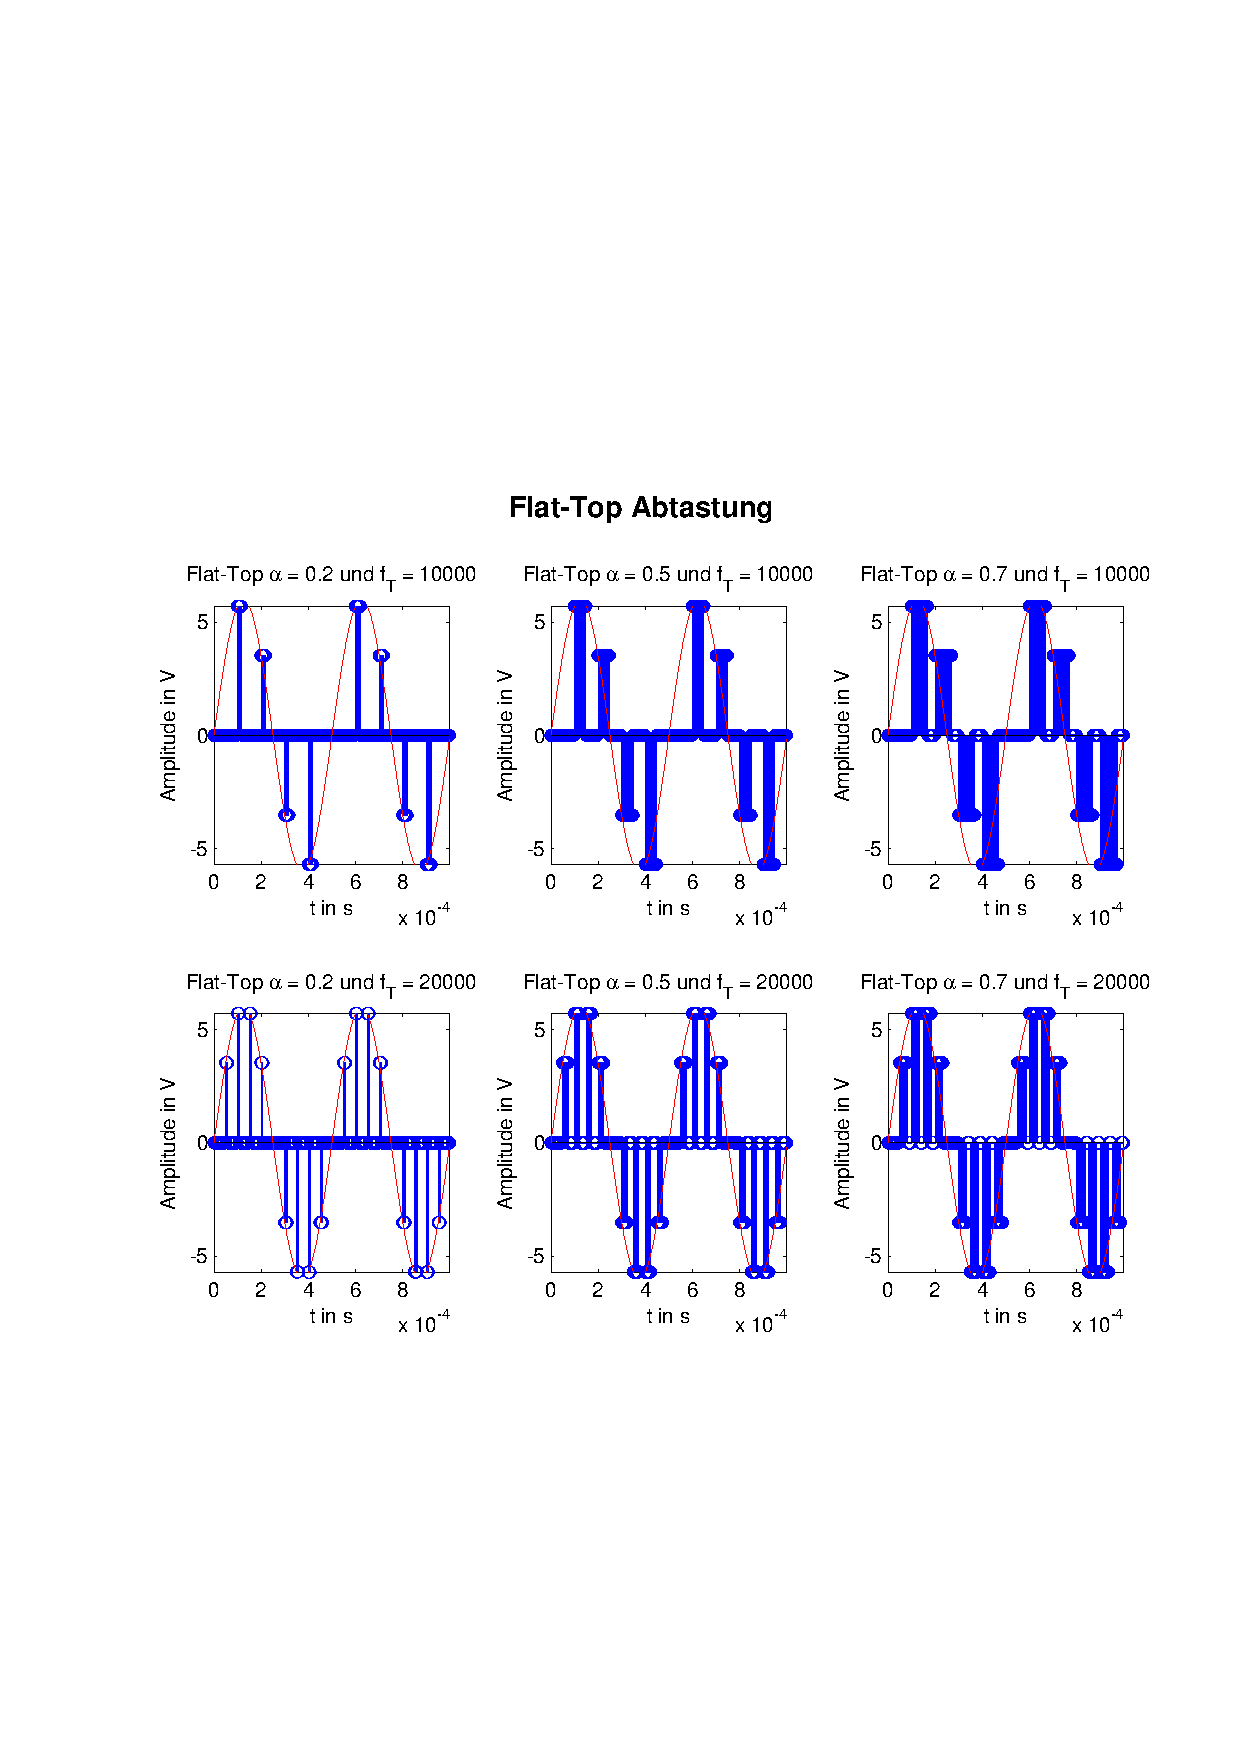
\includegraphics[scale=0.7, trim = 0cm 0cm 0cm 0cm,
        clip]{./Bilder/flat-top-zeit_3V}
            \caption{Zeitsignal mit flat-top-sampling und Abtastamplitude 3V}
  	    \end{figure}
  	    
  	    
  	    \begin{figure}[H]
    \centering
        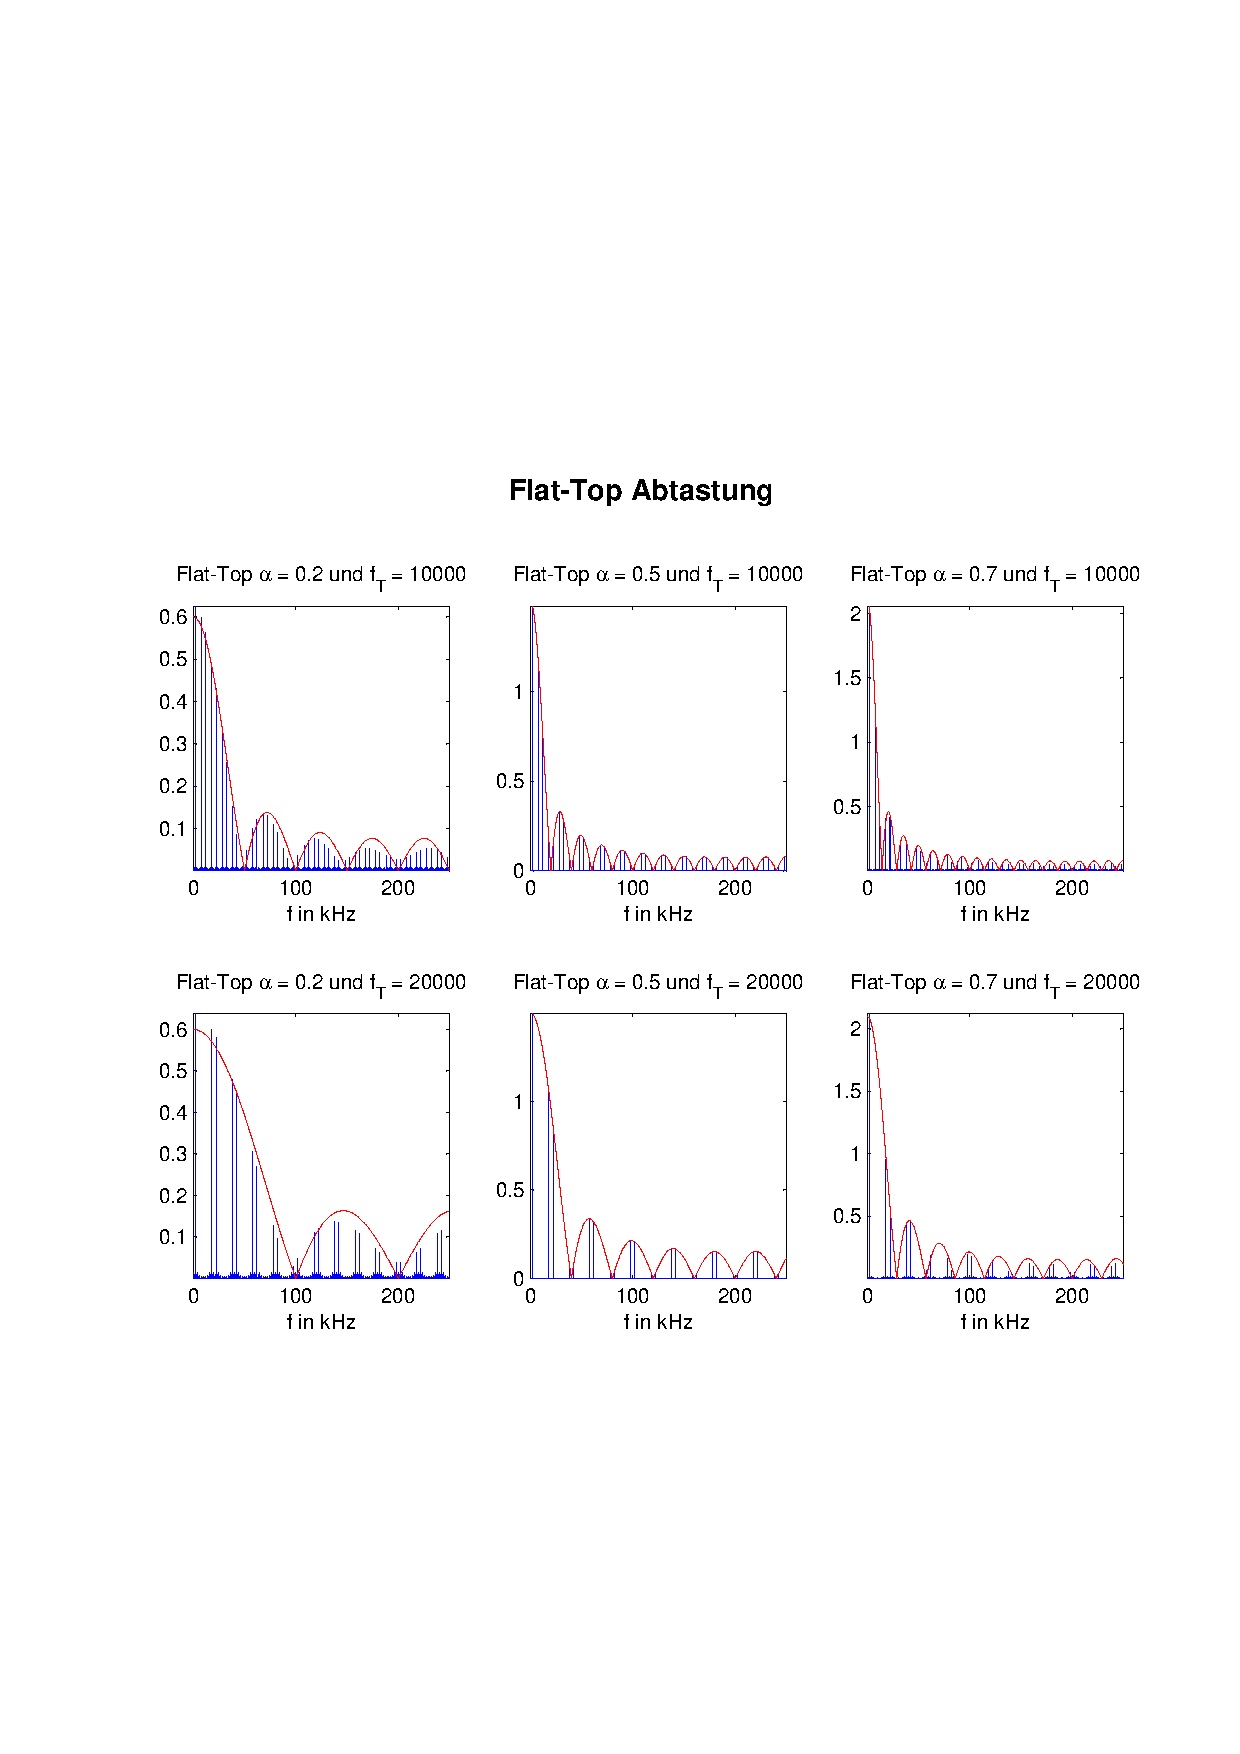
\includegraphics[scale=0.7, trim = 0cm 0cm 0cm 0cm,
        clip]{./Bilder/flat-top-freq_3V}
            \caption{Frequenzsignal mit flat-top-sampling und Abtastamplitude
            3V}
  	    \end{figure}
  	    
  	    
  	    Die Amplituden im Zeitsignal betragen wieder $6V$ und die Amplituden der
  	    Basisbänder nehmen die Werte $3V \cdot \alpha$ an. Ansonsten ist das
  	    Spektrum erneut deutlich verzerrter und alle anderen erwarteten
  	    Ergebnisse können auch hier wahrgenommen werden.
  	    
  	    
    \TODO{sind die Vorbereitungsaufgaben gut genug, dass wir sie beenden
    können?} 
    
    \end{quote}%subsection beenden

\end{quote}%Theorie beeanden
    
    \section{Labordurchführung}
    \begin{quote}
         \TODO{Durchführung schreiben}
   	\end{quote}%beende Labordurchführung
    	    
    
    \section{praktische Umsetzung}
    \begin{quote}
    Die praktische Umsetzung des Versuchs ist für beide Abtastverfahren gleich.
    
    \TODO{zu Ende bringen}
    \end{quote}%beende praktische Umsetzung
    
    
    \section{Auswertung}
    \begin{quote}    
        \TODO{Auswertung schreiben}
    \end{quote}%beende Auswertung
    
    \section{Zusammenfassung}
    \begin{quote}
    	\TODO{Zusammenfassung schreiben}
    \end{quote}%beende Zusammenfassung

%--------------------------------------------------------------------
%--------------------------------------------------------------------            

\TODO{Boris: öfter mal ein Überraschungsgeschenk für deine beste Freundin
besorgen!!}

%--------------------------------------------------------------------
%--------------------------------------------------------------------    


\begin{thebibliography}{999}
% \bibitem {AMohnetraeger} Prof. Dr.-Ing. Sikora, Thomas; Prof. Dr.-Ing. Noll, Peter: Einführung in die
% Nachrichtenübertragung, S.207




%Name, Vorname.; evtl. Name2, Vorname2.: Titel des Dokumentes
%oder Buches, Zeitschrift/Verlag/URL (Auflage, Erscheinungsort, -jahr), ggf. Seitenzahlen
% \bibitem {PasevalscheTheorem} \url{https://de.wikipedia.org/wiki/Parsevalsches_Theorem}, Zugriff
% 23.05.2012
\end{thebibliography}

\end{document}
